% \renewcommand{\theHsection}{A\arabic{section}}
% \appendixsiam
 

\appendix
% \newpage
% ~

% \newpage
% \section*{Appendix}
% \chapter{Appendix}
\section{Algorithm}

\subsection{Exploration}\label{appendix:alg:explora}
We summarize the comprehensive algorithmic procedure for exploration detailed in Section \ref{method:exploration} as presented in Algorithm \ref{algorithm:explorenreasoning}.

\begin{algorithm}[h]
	{
		{
			\SetVline
			\small
			\caption{{\small{Exploration}}}\label{algorithm:explorenreasoning}
            
			\Input{Question subgraph ($\mathcal{G}_q$), source KG ($\mathcal{G}$),question and split question ($Q = q$ + $q_{split}$), topic entities ($Topic(q)$), LLM indicator ($I_{\text{LLM}}$), predict depth ($D_{\text{predict}}$), maximum depth ($D_{\max}$),  maximum width ($W_{\max}$), and path pruning case ($case$)}
			\Output{PoG answers ($a(q)$), final reasoning path ($Paths_f(q)$)}
            % \State{$T_d^+ \leftarrow$ Obtain positive $k$-truss with smallest query distance $d$ containing $Q$ in Algorithm~\ref{alg_local}}
            % \setstretch{1.25}
            % \tcc{\textcolor{blue}{Start with topic entity path exploration}}
            \vspace{1mm}
            
            \CmtState{\\$List_{T} \leftarrow$ \text{Reorder}($Topic(q), I_{\text{LLM}}$), $D \leftarrow$ min($D_{\text{predict}}, D_{\max}$)} 
            {\textbf{Start with topic entity path exploration}}
            % \State{$D \leftarrow$ min($D_{\text{predict}}, D_{max}$)}
            
            \While{ $D \leq D_{\max}$} {
                \State{$Paths_t \leftarrow \text{EntityPathFind}$ ($List_{T},D$,$\mathcal{G}_q$)}
                \State{$\text{PathPruning}(Paths_t, Q, I_{\text{LLM}}, W_{\max},D_{\max}, List_{T}, case)$}
                \State{$Answer, Paths_{T} \leftarrow \text{QuestionAnswering}(Paths_t, Q, I_{\text{LLM}})$}

                
                \State{\textbf{if}  $\texttt{"\{Yes\}"} \text{ in } Answer$  \textbf{then} \textbf{return} $Answer, Paths_{T}$;\\ \textbf{else} $D \leftarrow D + 1$}
			}
    % \State{\textbf{if} $Answer$ = True \textbf{then} \textbf{return} $Answer, Paths_{T}$ }

% \textcolor{blue}{\tcc{LLM supplement path exploration procedure}}
\vspace{1mm}
\CmtState{\\$Paths_s \leftarrow []$}{\textbf{LLM supplement path exploration procedure} }

\State{$ Predict(q) \leftarrow  $SupplementPrediction($Paths_T, Q, I_{\text{LLM}}$)} 
\ForEach{ $e,I_{sup(e)} \in Predict(q)$} {
    % \State{$List_{S} \leftarrow $ $List_{T} +e$ }
    
    \State{$List_{S} \leftarrow $ Reorder ($List_{T} +e, I_{sup(e)}$)}
    \State{$Paths_s' \leftarrow \text{EntityPathFind}$ ($List_{S},D_{\max}$,$\mathcal{G}_q$)}
    \State{$Paths_s \leftarrow  Paths_s + \text{FuzzySelect}$ ($Paths_s', I_{sup(e)}, W_{\max}$)}
    }

    \State{$ \text{PathPruning}(Paths_s, Q, I_{\text{LLM}}, W_{\max},D_{\max}, List_{S}, case)$}
    \State{$Answer, Paths_{S} \leftarrow \text{QuestionAnswering}(Paths_s, Q, I_{\text{LLM}})$}

    % \State{$Answer, Paths_{S} \leftarrow \text{Reasoning}(Paths_s, Q, I_{\text{LLM}})$}
   
   


    \State{\textbf{if} \texttt{"\{Yes\}"} in $Answer$ \textbf{then} \textbf{return} $Answer, Paths_{S}$ }
    

% \textcolor{blue}{\tcc{Node expand exploration procedure}}
\vspace{1mm}

   \CmtState{\\$Visted \leftarrow \emptyset$, $D\leftarrow1$, $Paths_e \leftarrow Paths_{T} +Paths_{S} $}{\textbf{Node expand exploration procedure} }
   % \State{$Paths_e \leftarrow Paths_{T} +Paths_{S} $}
   % \If{$|Paths_e| > W_{max}$} {
   % $\text{PathsPruning}(Paths_e, Q, I_{\text{LLM}}, W_{max}, D_{max}, List_{T}, case)$;}
   \State{$\text{PathPruning}(Paths_e, Q, I_{\text{LLM}}, W_{\max}, D_{\max}, List_{T}, case)$;}

   \While{$D\leq D_{\max}$} {
    % \State{$Entities \leftarrow$ ExtractEntity($Paths_e$)}
    \ForEach{$e \in \text{ExtractEntity}(Paths_e) \land e \notin Visted$} {
        \State{$Related\_edges = \text{Find\_1\_hop\_Edges}(\mathcal{G}, e)$}
        \State{$Paths_e \leftarrow \text{MergeTogether}(Paths_e, Related\_edge)$}

        
        % \State{$Visted = Visted \cup e$; $D\leftarrow D+1$}
    }
    \State{$\text{PathPruning}(Paths_e, Q, I_{\text{LLM}}, W_{\max},D_{\max},List_{T}, case)$}
    \State{$Answer, Paths_{e} \leftarrow \text{QuestionAnswering}(Paths_e, Q, I_{\text{LLM}})$}
    % \State{\textbf{if} $Answer$ = True \textbf{then} \textbf{return} $Answer, Paths_{e}$ }
    \State{\textbf{if} $ \texttt{"\{Yes\}"} \text{ in } Answer$  \textbf{then} \textbf{return} $Answer, Paths_{e}$;\\ \textbf{else} $Visted \leftarrow Visted \cup e$; $D\leftarrow D+1$}
}

    \State{
    $Paths_l \leftarrow Paths_T+Paths_S+Paths_E$
    }
    \State{
    $ \text{PathPruning}(Paths_l, Q, I_{\text{LLM}}, W_{\max},D_{\max}, List_{T},case)$}
    
    \State{$Answer,Paths_L \leftarrow \text{QuestionAnsweringFinal}(Paths_l, Q, I_{\text{LLM}})$}
    \State{\textbf{Return} $Answer,Paths_L$}
    % \textbf{Procedure} PathsReasoning$(Paths_{t}, Q, I)$\\
    % \SetVline
    % \small
    % % \If{$v \neq Q$}{
    % \StateCmt{$Paths_{f} \leftarrow \text{PathPathsPruning} (Paths_{t}, Q,  I)$}{Utilizing Bi}
    
    
    % \State{$Answer, Paths_{f} \leftarrow \text{QA}(Paths_{f}, Q,  I_{\text{LLM}})$}
}
}
\end{algorithm}
\newpage
\subsection{Path Pruning}\label{appendix:alg:pathpruning}
We summarize the comprehensive algorithmic procedure of path pruning detailed in Section \ref{method:3pathprune} as presented in Algorithm \ref{algorithm:PathsPruning}. 

\begin{algorithm}[h]
	{
		{
			\SetVline
			\small
			\caption{{\small{PathPruning}}}\label{algorithm:PathsPruning}
            
			\Input{Candidate paths($Paths_{c}$), question and split question ($Q = q+ q_{split}$), indicator ($I$), maximum width ($W_{\max}$), maximum depth ($D_{\max}$), entity list ($list$)}
			\Output{Pruned candidate paths ($Paths_{c}$)}
            % \State{$T_d^+ \leftarrow$ Obtain positive $k$-truss with smallest query distance $d$ containing $Q$ in Algorithm~\ref{alg_local}}
            % \setstretch{1.25}
            % \tcc{\textcolor{blue}{Start with topic entity path exploration}}
            \If{Case = \texttt{Fuzzy Selection Only}}
            {
            \State{$ \text{FuzzySelect}(Paths_{c},Q, I,W_{\max})$}}
            \ElseIf{Case = \texttt{Fuzzy + Precise Path Selection}}
            {
            \State{$ \text{FuzzySelect}(Paths_{c},Q, I,W_{1})$}
            \State{$ \text{PrecisePathSelect}(Paths_{c},Q, I,W_{\max})$}
            } 
            \ElseIf{Case = \texttt{Fuzzy + Branch Reduced Selection}}
            {
            \State{$ \text{FuzzySelect}(Paths_{c},Q, I,W_{1})$}
            \State{$ \text{BranchReduceSelect}(Paths_{c},Q, I,W_{\max},D_{\max},list)$}
            
            }
            \ElseIf{Case = \texttt{Fuzzy + Branch Reduced + Precise Path}}
            {
            \CmtState{$ \text{FuzzySelect}(Paths_{c},Q, I,W_{1})$} 
            {case = 3-Step Beam Search}
            \State{$ \text{BranchReduceSelect}(Paths_{c},Q, I,W_{2},D_{\max},list)$}
            \State{$ \text{PrecisePathSelect}(Paths_{c},Q, I,W_{\max})$}
            
            }
        % \State{\textbf{Return} $Paths_{c}$}
            \vspace{1mm}
            \textbf{Procedure} BranchReduceSelect$(Paths_{c}, Q, I, W, D_{\max}, list)$\\
            \SetVline
            \small
            % \If{$v \neq Q$}{
            \State{$D \leftarrow 1$, $Paths_{e} \leftarrow \emptyset$}
            % \State{}
            
            \While{$|Paths_{c}| \geq W \land D \leq D_{\max}$} {

                
            \ForEach{$e\in list$} {
                
                \State{$Paths_{e} \leftarrow Paths_{e} \cup \text{ExtractHeadSteps}(Paths_{c}, e, D)$}
            }
            \If{$|Paths_{e}| > W$} {
                \State{$ \text{PrecisePathSelect}(Paths_{e},Q, I,W)$}
            
                \State{$Paths_{c} \leftarrow \text{IntersectMatchUpdate}(Paths_{e}, Paths_{c})$}
                \State{$Paths_{e} \leftarrow \emptyset$}
            }
            \State{$D\leftarrow D+1$}
        }

            \State{\textbf{if} $|Paths_{c}| > W$ \textbf{then} $ \text{PrecisePathSelect}(Paths_{c},Q, I,W)$}

    }
    }
\end{algorithm}




\newpage
\section{Experiment}\label{appendix:expriment}

\subsection{Additional Ablation Study}\label{appendix:Ablation}


\myparagraph{Compare the effect of different beam search strategies} As introduced in Section \ref{method:3pathprune}, PoG supports various beam search strategies, ranging from non-reliant to fully reliant on LLMs, selectable in a user-friendly manner. To evaluate the computational cost and performance, we test four cases outlined in Algorithm \ref{algorithm:PathsPruning}. In the \texttt{3-Step Beam Search} case, we set $W_2 = 20$ for internal narrowing. The \texttt{Fuzzy Selection} approach, as described in Section \ref{method:3pathprune}, utilizes all candidate paths and a LLM-generated indicator for encoding and comparison.
% We measure accuracy, average LLM calls, and average token input to the LLM API during the path pruning phase to measure efficiency and effectiveness
% We report accuracy, average LLM calls, and average token input during the path pruning phase for each beam search strategy in Table \ref{fig:ablation:vary_beamsearch} for PoG. 
% The experiment result of PoG-E is detailed in Table \ref{fig:ablation:vary_beamsearch_pog-e} of Appendix \ref{appendix:Ablation}. 
We report accuracy, average LLM calls in total, and average token input during the path pruning for each beam search strategy applied to PoG and PoG-E in Table \ref{fig:ablation:vary_beamsearch} and Table \ref{fig:ablation:vary_beamsearch_pog-e}.
These results indicate that PoG/PoG-E with \texttt{Fuzzy and Precise Path Selection} achieves the highest accuracy. Additionally, the \texttt{BranchReduced Selection} method, which leverages the graph structure, not only delivers excellent results but also reduces token usage by over 50\% (65\%) with only a ±2\% (±4.3\%) difference in accuracy on PoG (PoG-E) compared to the best-performing strategy. Furthermore, the \texttt{Fuzzy Selection} method, which employs lightweight models instead of relying solely on LLMs, also demonstrates strong performance. These results validate the effectiveness of our beam search strategies and underscore the importance of structure-based faithful path reasoning. 
% The performance result of PoG-E is shown in Table \ref{fig:ablation:vary_beamsearch_pog-e}.
% Please add the following required packages to your document preamble:
% \usepackage{booktabs}
% \usepackage[normalem]{ulem}
% \useunder{\uline}{\ul}{}


\begin{table}[h]
\caption{Performance comparison of PoG with different beam search methods on CWQ and WebQSP.}\label{fig:ablation:vary_beamsearch}
\begin{tabular}{@{}llcc@{}}
% \small
\toprule
\textbf{PoG}              & \textbf{Evaluation} & \textbf{CWQ}  & \textbf{WebQSP} \\ \midrule
w/ Fuzzy Selection        & Accuracy           & 57.1          & 86.4           \\
                          & Token Input         & -             & -               \\
                          & LLM Calls       & 6.8           & 6.5             \\ \midrule
w/ Fuzzy and              & Accuracy           & 79.3          & {\ul 93.0}     \\
BranchReduced Selection & Token Input         & 101,455       & 328,742         \\
                          & LLM Calls       & 9.7         & 9.3             \\ \midrule
w/ Fuzzy and              & Accuracy           & \textbf{81.4} & \textbf{93.9}   \\
Precise Path Selection    & Token Input         & 216,884       & 617,448         \\
                          & LLM Calls       & 9.1           & 7.5             \\ \midrule
w/ 3-Step Beam Search    & Accuracy           & {\ul 79.8}    & 91.9            \\
                          & Token Input         & 102,036       & 369,175         \\
                          & LLM Calls       & 8.8           & 9.0               \\ \bottomrule
\end{tabular}
\end{table}

\newpage
\myparagraphquestion{How do summary prompts affect} 
Inspired by GoT \cite{besta2024graphGoT}, we utilize summary prompts to reduce LLM hallucinations and decrease computational costs. To evaluate their impact, we conduct an ablation study comparing PoG and PoG-E with and without path summarization. We measure both accuracy and average token input to the LLM API during the path pruning phase to measure efficiency and effectiveness.
The results, present in Tabel \ref{fig:ablation:summ_prompt}, show that using graph summaries increases accuracy by up to 10\% on the CWQ dataset with PoG-E, while reducing token input by up to 36\% on WebQSP. These results indicate hat path summarization effectively minimizes LLM hallucinations, enhances the LLM's understanding of the explored paths, facilitates answer retrieval, enables earlier termination of the reasoning process, and reduces costs.
\begin{table}[h]

\caption{Performance comparison of PoG-E with different beam search methods among CWQ and WebQSP datasets.}\label{fig:ablation:vary_beamsearch_pog-e}
\begin{tabular}{@{}llcc@{}}
\toprule
\textbf{PoG-E}          & \textbf{Evaluation} & \textbf{CWQ}  & \textbf{WebQSP} \\ \midrule
w/ FuzzySelect          & Accuracy           & 62.31         & 82.3            \\
                        & Token Input         & -             & -               \\
                        & Ave LLM Calls       & 6             & 6.3             \\ \midrule
w/ Fuzzy and            & Accuracy           & 71.9          & 88.4            \\
BranchReduced Selection & Token Input         & 128,407       & 371,083         \\
                        & Ave LLM Calls       & 9.4           & 9.1             \\ \midrule
w/ Fuzzy and            & Accuracy           & \textbf{80.4} & \textbf{91.4}   \\
Precise Path Selection  & Token Input         & 344,747       & 603,261         \\
                        & Ave LLM Calls       & 8.3           & 7.4             \\ \midrule
w/ 3-Step Beam Search  & Accuracy           & {\ul 73.87}   & {\ul 89.4}      \\
                        & Token Input         & 120,159       & 411,283         \\
                        & Ave LLM Calls       & 8.3           & 9.1             \\ \bottomrule
\end{tabular}

\end{table}

\begin{table}[h]
\caption{Performance comparison of PoG and PoG-E with and without path summarizing on CWQ and WebQSP datasets.}\label{fig:ablation:summ_prompt}
\begin{tabular}{@{}llcc@{}}
\toprule
\textbf{Method}      & \textbf{Evaluation} & \textbf{CWQ} & \textbf{WebQSP} \\ \midrule
\textbf{PoG}         &                     &              &                 \\
w/ Path Summarizing   & Accuracy           & \textbf{81.4 }        & \textbf{93.9}            \\
                     & Token Input         & 216,884      & 297,359         \\
w/o Path Summarizing & Accuracy           & 74.7         & 91.9            \\
                     & Token Input         & 273,447      & 458,545         \\ \midrule
\textbf{PoG-E}       & \textbf{}           & \textbf{}    & \textbf{}       \\
w/ Path Summarizing   & Accuracy           & \textbf{80.4 }        & \textbf{91.4}            \\
                     & Token Input         & 314,747      & 273,407         \\
w/o Path Summarizing & Accuracy           & 70.4         & 90.4            \\
                     & Token Input         & 419,679      & 428,545         \\ \bottomrule
\end{tabular}
\end{table}
% Please add the following required packages to your document preamble:
% \usepackage{booktabs}


% Please add the following required packages to your document preamble:
% \usepackage{booktabs}
% \usepackage[normalem]{ulem}
% \useunder{\uline}{\ul}{}

\newpage
\subsection{Reasoning Faithfulness Analysis}\label{appendix:exp:reasoning_faithful}
\myparagraph{Overlap ratio between explored paths and ground-truth paths}
We analyzed correctly answered samples from three datasets to investigate the overlap ratio between the paths $P$ explored by PoG and the ground-truth paths $S$ in SPARQL queries. The overlap ratio is defined as the proportion of overlapping relations to the total number of relations in the ground-truth SPARQL path:

\[
Ratio(P) = \frac{|Relation(P) \cap Relation(S)|}{|Relation(S)|},
\]

\noindent where $Relation(P)$ denotes the set of relations in path $P$.
Figure \ref{fig:exp:overlap} illustrates the distribution of questions across different overlap ratios. For the WebQSP dataset, PoG achieves the highest proportion of fully overlapping paths with the ground truth, reaching approximately 60\% accuracy. In contrast, PoG-E applied to the GrailQA dataset shows the highest proportion of paths with up to 70\% non-overlapping relations, indicating that PoG-E explores novel paths to derive the answers.
The different results between PoG and PoG-E are due to PoG-E's strategy of randomly selecting one related edge from each clustered edge. This approach highlights the effectiveness of our structure-based path exploration method in generating diverse and accurate reasoning paths.


\begin{figure}[h]
    % \centering
    \begin{subfigure}{0.495\linewidth}
           \centering
           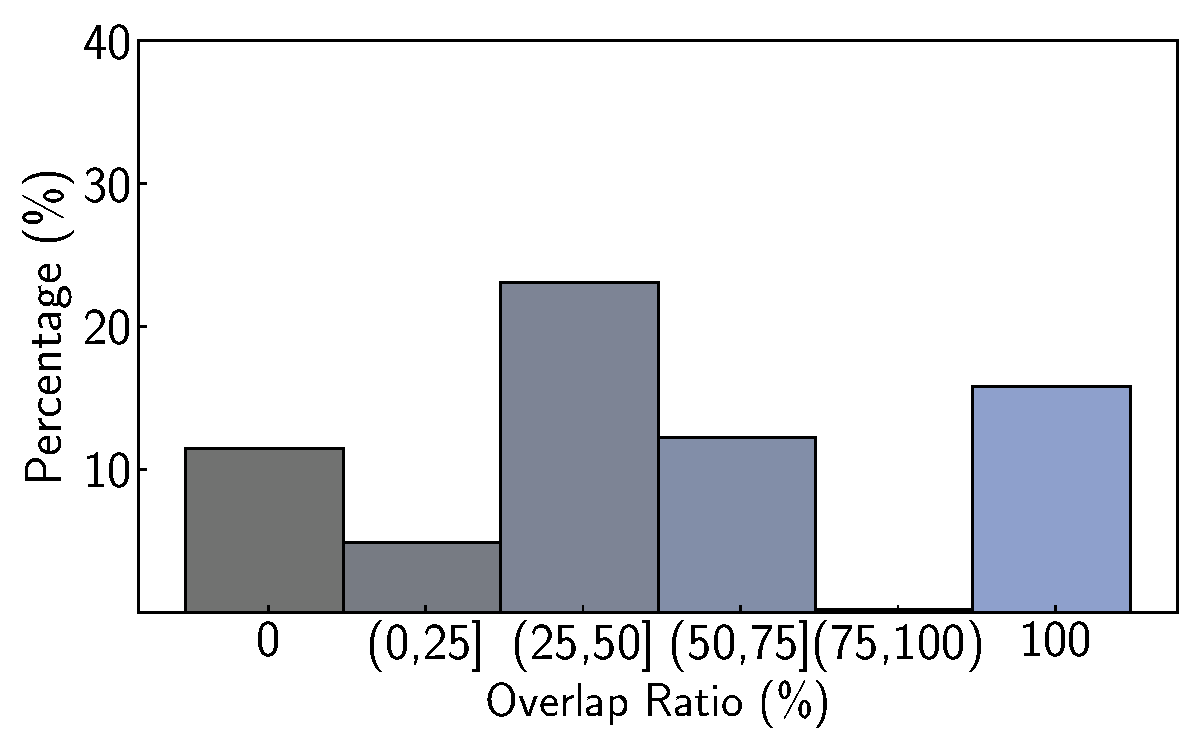
\includegraphics[width=1\linewidth]{graphs/path_overlap_cwq_pog_1.pdf}
           
           \caption{CWQ (PoG)}
            \label{fig:a}
    \end{subfigure}
    \begin{subfigure}{0.495\linewidth}
           \centering
           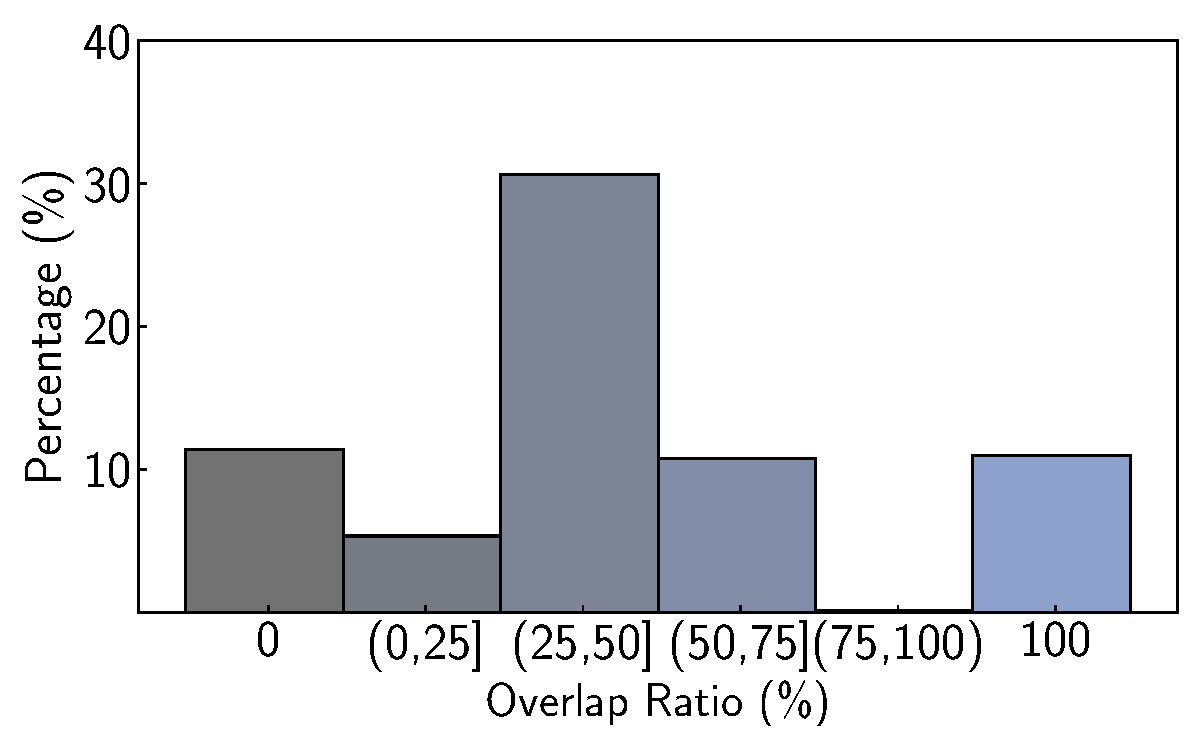
\includegraphics[width=1\linewidth]{graphs/path_overlap_cwq_pog_e.pdf}
           
           \caption{CWQ (PoG-E)}
            \label{fig:a}
    \end{subfigure}
    \begin{subfigure}{0.495\linewidth}
           \centering
           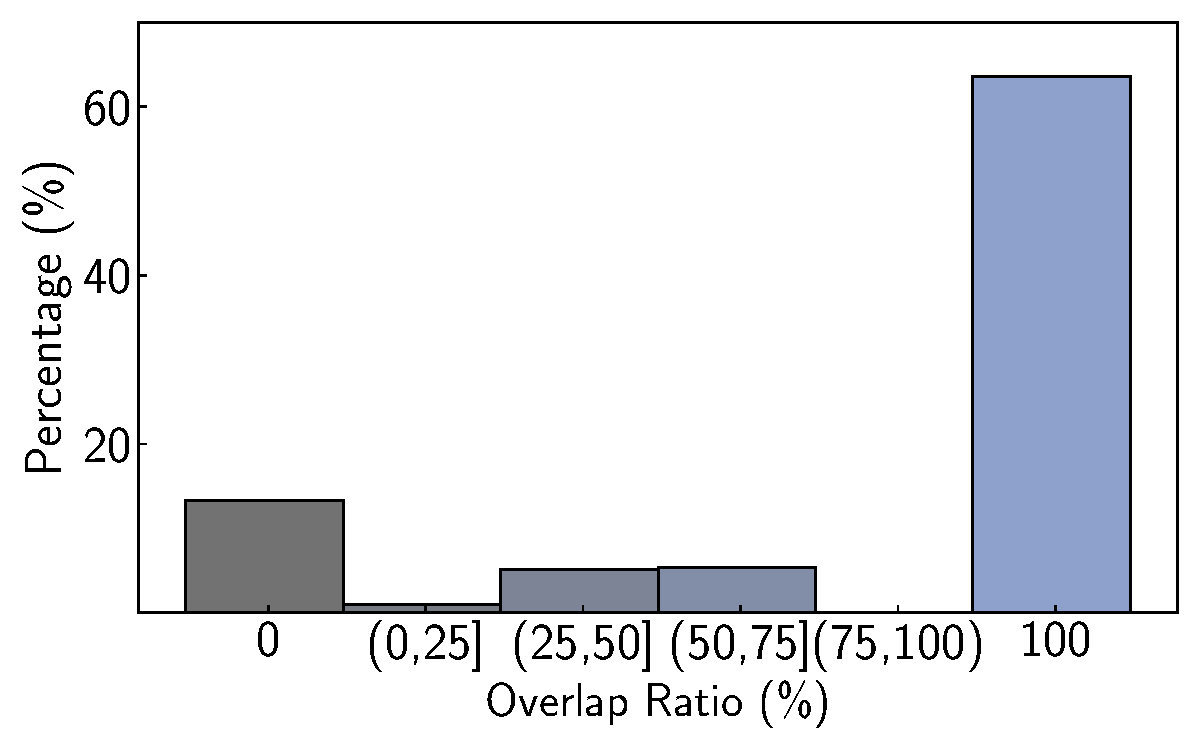
\includegraphics[width=1\linewidth]{graphs/path_overlap_webqsp_pog_1.pdf}
           
           \caption{WebQSP (PoG)}
            \label{fig:a}
    \end{subfigure}
    \begin{subfigure}{0.495\linewidth}
           \centering
           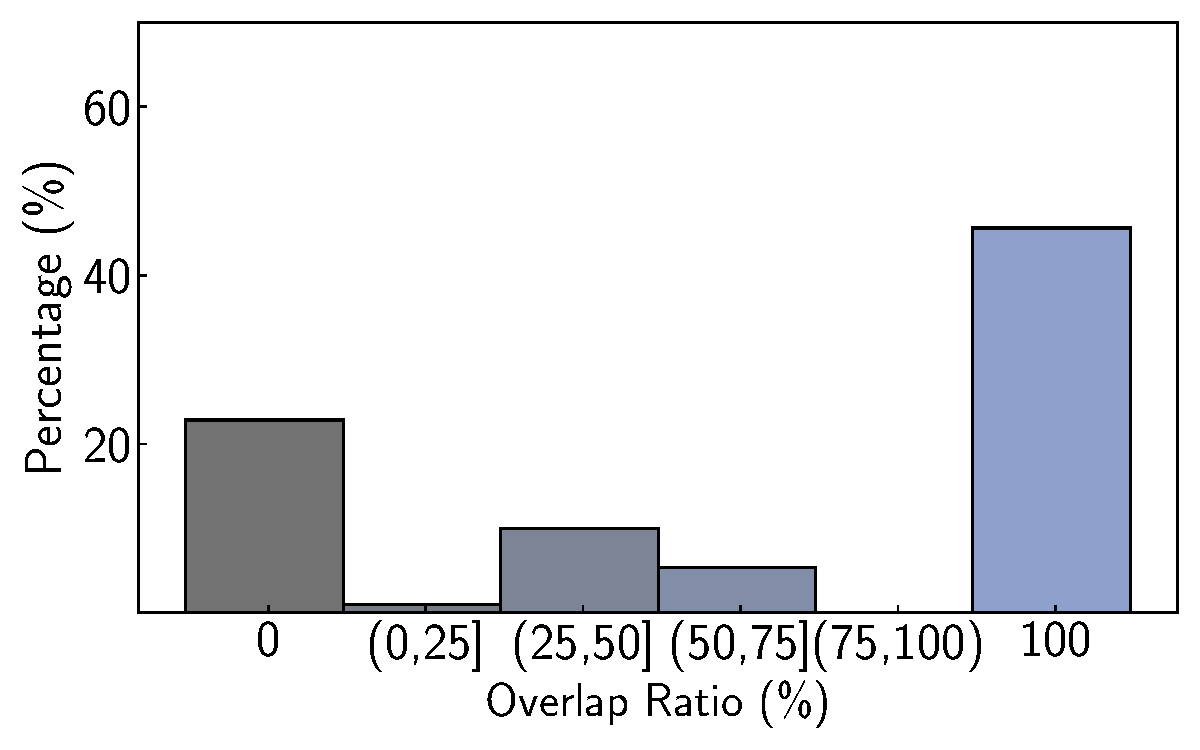
\includegraphics[width=1\linewidth]{graphs/path_overlap_webqsp_pog_e.pdf}
           
           \caption{WebQSP (PoG-E)}
            \label{fig:a}
    \end{subfigure}
    \begin{subfigure}{0.495\linewidth}
           \centering
           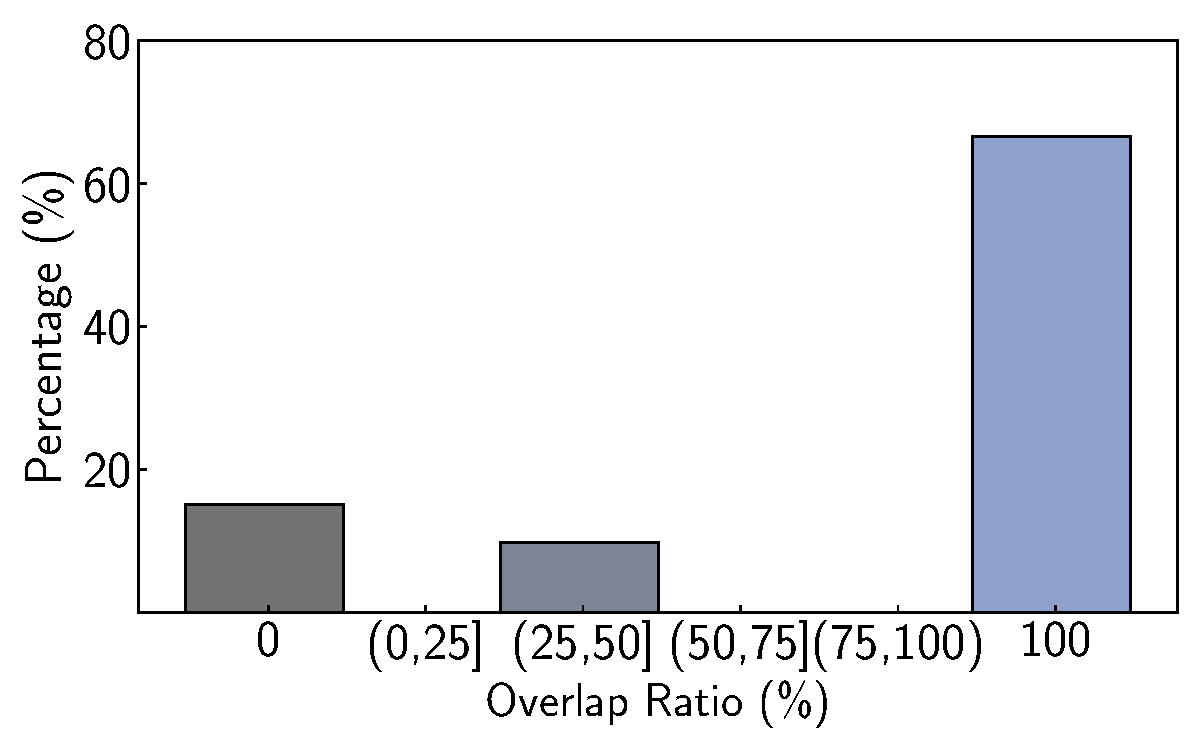
\includegraphics[width=1\linewidth]{graphs/path_overlap_grailqa_pog_1.pdf}
           
           \caption{GrailQA (PoG)}
            \label{fig:a}
    \end{subfigure}
    \begin{subfigure}{0.495\linewidth}
           \centering
           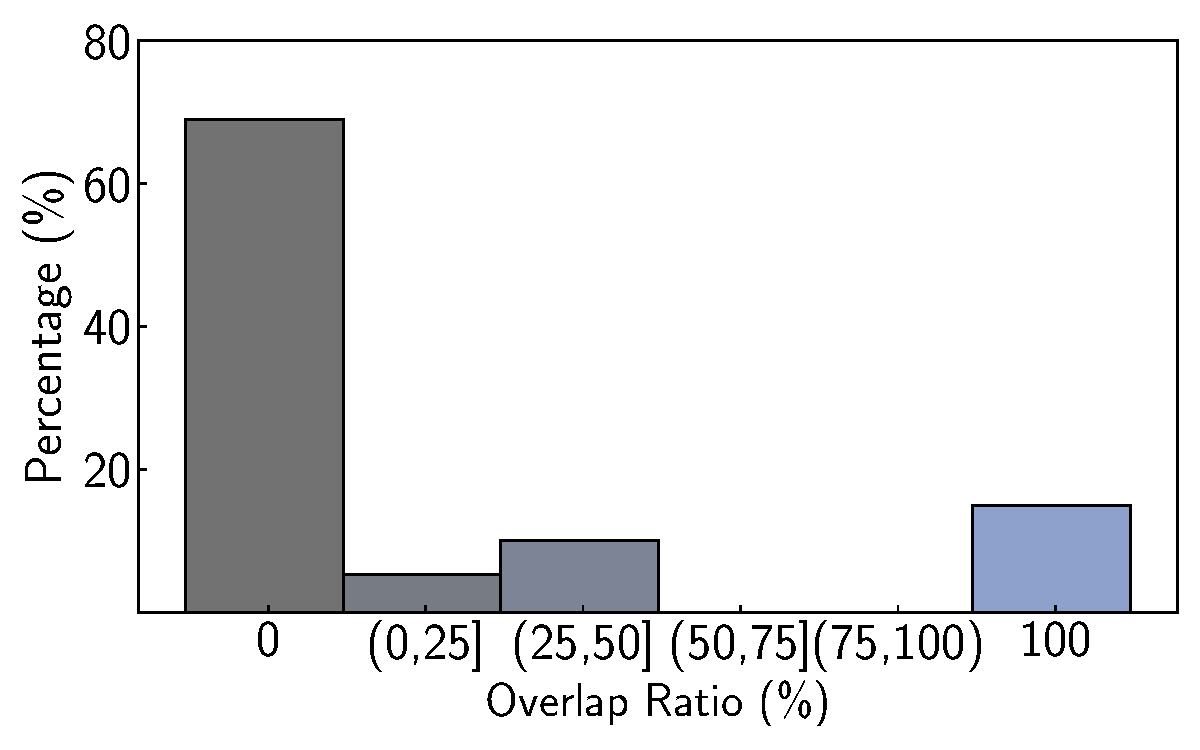
\includegraphics[width=1\linewidth]{graphs/path_overlap_grailqa_pog_e.pdf}
           
           \caption{GrailQA (PoG-E)}
            \label{fig:a}
    \end{subfigure}
    
\caption{ The path overlap ratio of PoG and PoG-E among CWQ, WebQSP, and GrailQA datasets.}\label{fig:exp:overlap}
    
\end{figure}

\newpage
\myparagraph{Evidence of answer exploration sources}
We conduct an analysis of correctly answered samples from three datasets to investigate the sources of evidence used by the LLM in generating answers, as illustrated in Figure \ref{fig:exp:answer_gen_by}. Specifically, we categorize all generated answers into three cases: KG only, LLM-inspired KG, and KG-inspired LLM.
In the \textit{KG only} scenario, answers are generated solely based on KG paths. The \textit{LLM-inspired KG} case involves the LLM predicting an answer using its inherent knowledge and subsequently using the KG to verify its correctness. Conversely, in the \textit{KG-inspired LLM} case, the paths generated by the KG are insufficient to reach the answer, and the LLM supplements the reasoning using its inherent knowledge.
As shown in the figure, up to 14\% of answers are generated through the KG-inspired LLM approach, and up to 9\% involve LLM-inspired KG path supplementation. Compared to previous work that integrates LLM inherent knowledge with KG data\cite{tog1.0sun2023think}, PoG more effectively leverages the strengths of both sources. These results demonstrate that PoG is a faithful reasoning method that primarily relies on KG-based reasoning while being supplemented by the LLM, ensuring both accuracy and interpretability in answer generation.
\begin{figure}[h]
    % \centering
    % 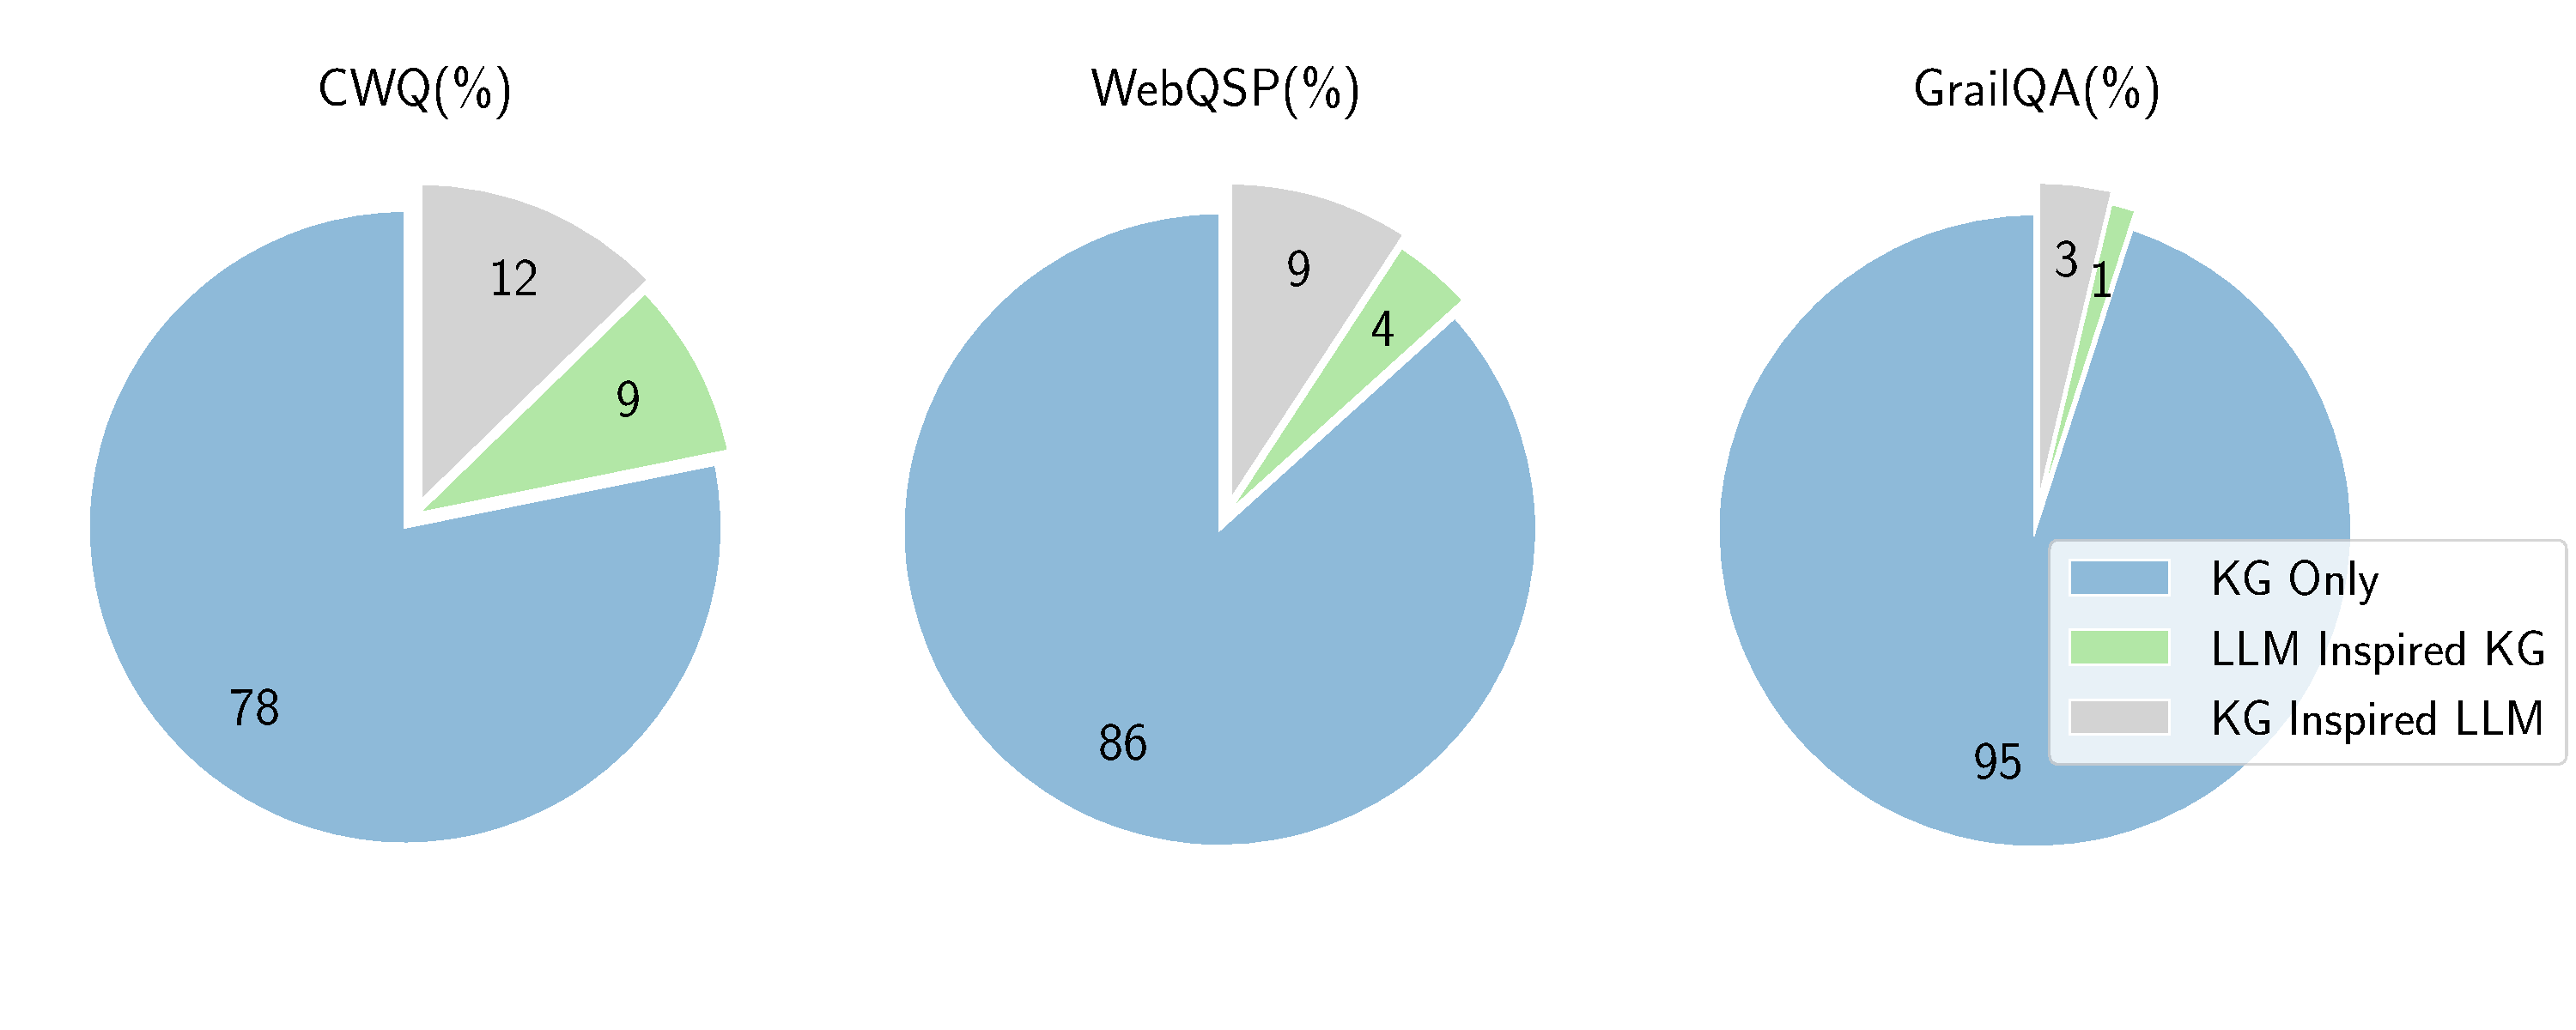
\includegraphics[width=0.34\linewidth]{graphs/answer_precentage_PoG.pdf}
    % \vspace{-5mm}
    % \caption{The lengths of the ground-truth Sparql queries within the CWQ and WebQSP datasets.}
    % \label{fig:enter-label}
    % \centering
    \begin{subfigure}{1\linewidth}
           \centering
           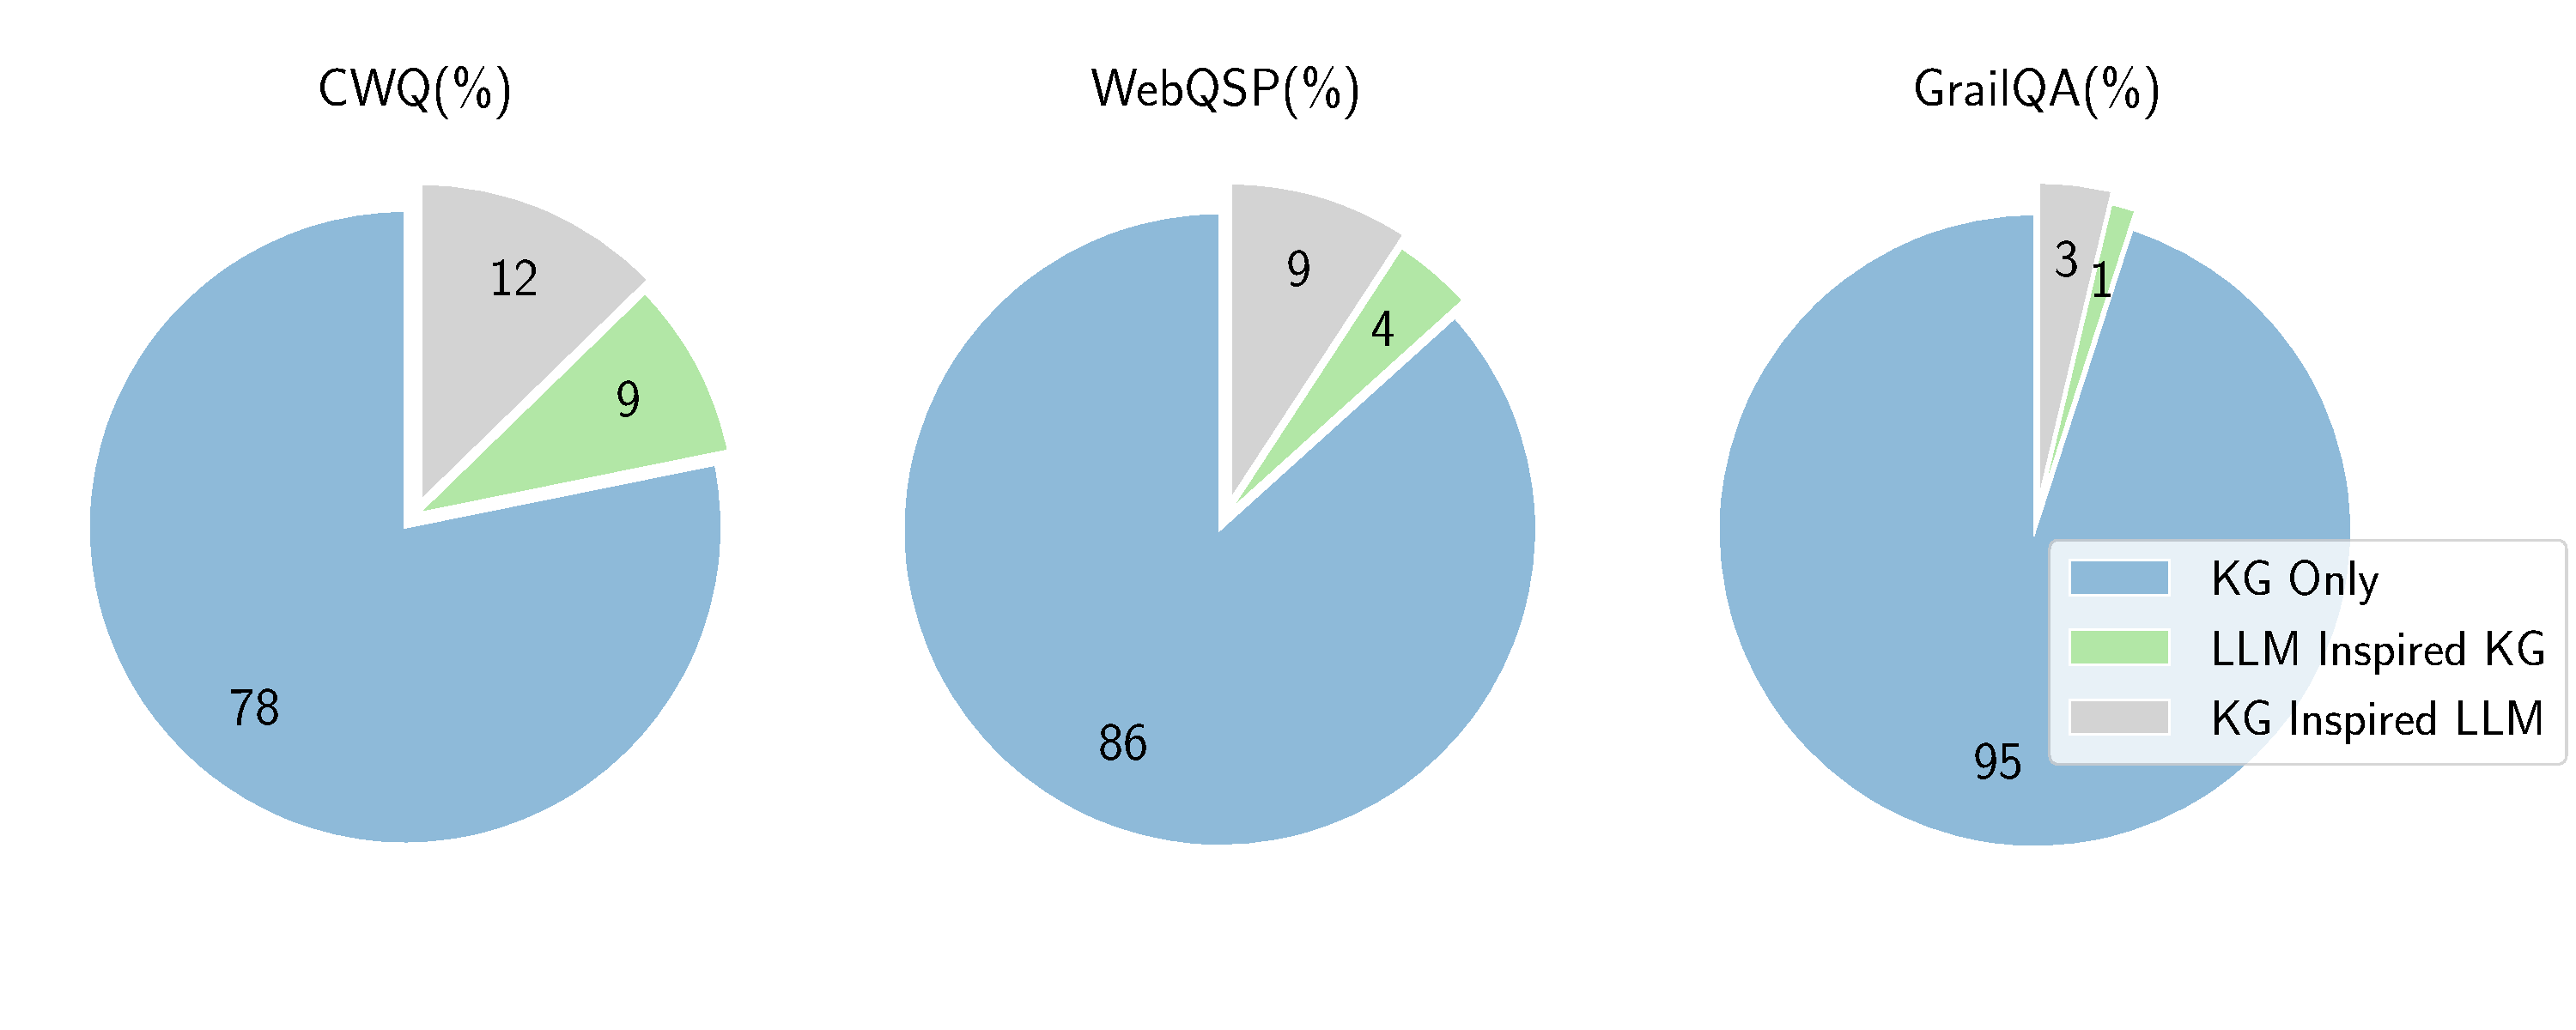
\includegraphics[width=1\linewidth]{graphs/answer_precentage_PoG.pdf}
           
           \caption{PoG}
            \label{fig:a}
    \end{subfigure}
    \begin{subfigure}{0.99\linewidth}
           \centering
           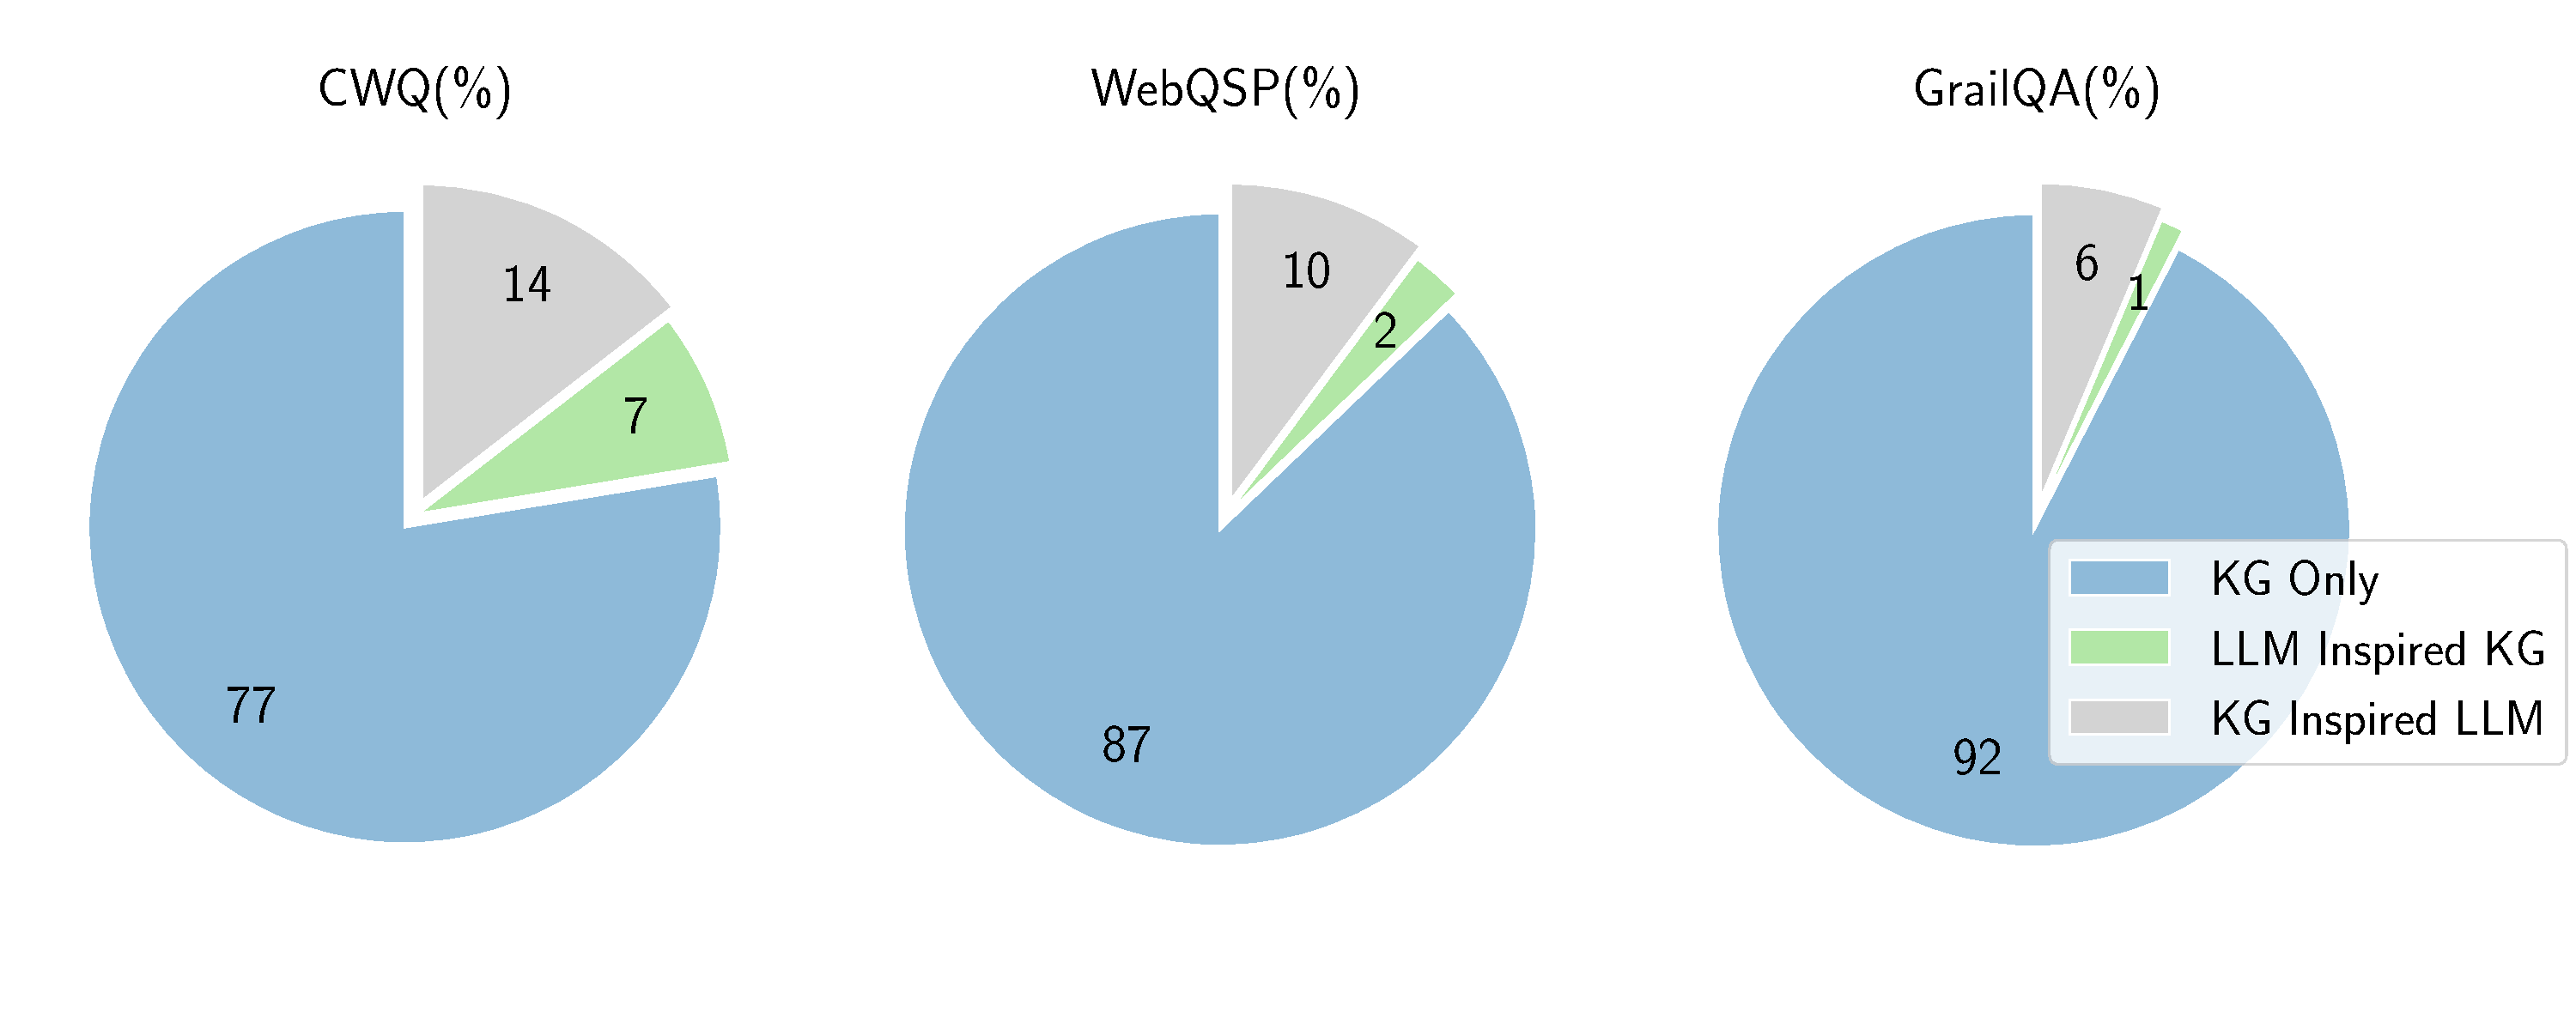
\includegraphics[width=1\linewidth]{graphs/answer_precentage_PoG_e.pdf}
           
           \caption{PoG-E}
            \label{fig:a}
    \end{subfigure}
    
\caption{The proportions of answer evidence of PoG and PoG-E among CWQ, WebQSP, and GrailQA datasets.}\label{fig:exp:answer_gen_by}
\end{figure}




\newpage
\subsection{Error Analysis}\label{appendix:exp:error_analysis}

% \myparagraph{Error analysis}
To further analyze the integration of LLMs and KGs, we conduct an error analysis on the CWQ, WebQSP, and GrailQA datasets. We categoriz errors into four types: (1) answer generation error, (2) refuse error, (3) format error, and (4) other hallucination errors. Note that answer generation error occurs when PoG provides an accurate reasoning path, but the LLM fails to extract the correct answer from it.
The distribution of these error types is illustrated in Figure \ref{fig:exp:error_analysis}. The results indicate that using more powerful LLMs reduces the number of "other hallucination errors," "refuse errors," and "answer generation errors," as the model offers enhanced reasoning capabilities based on the retrieved data. Specifically, the reduction in "answer generation errors" shows the reasoning paths provided by PoG are effectively utilized by more advanced LLMs. However, we observe an increase in "format errors" with more powerful LLMs, which may be attributed to their greater creative flexibility.
\begin{figure}[h]
    \centering
    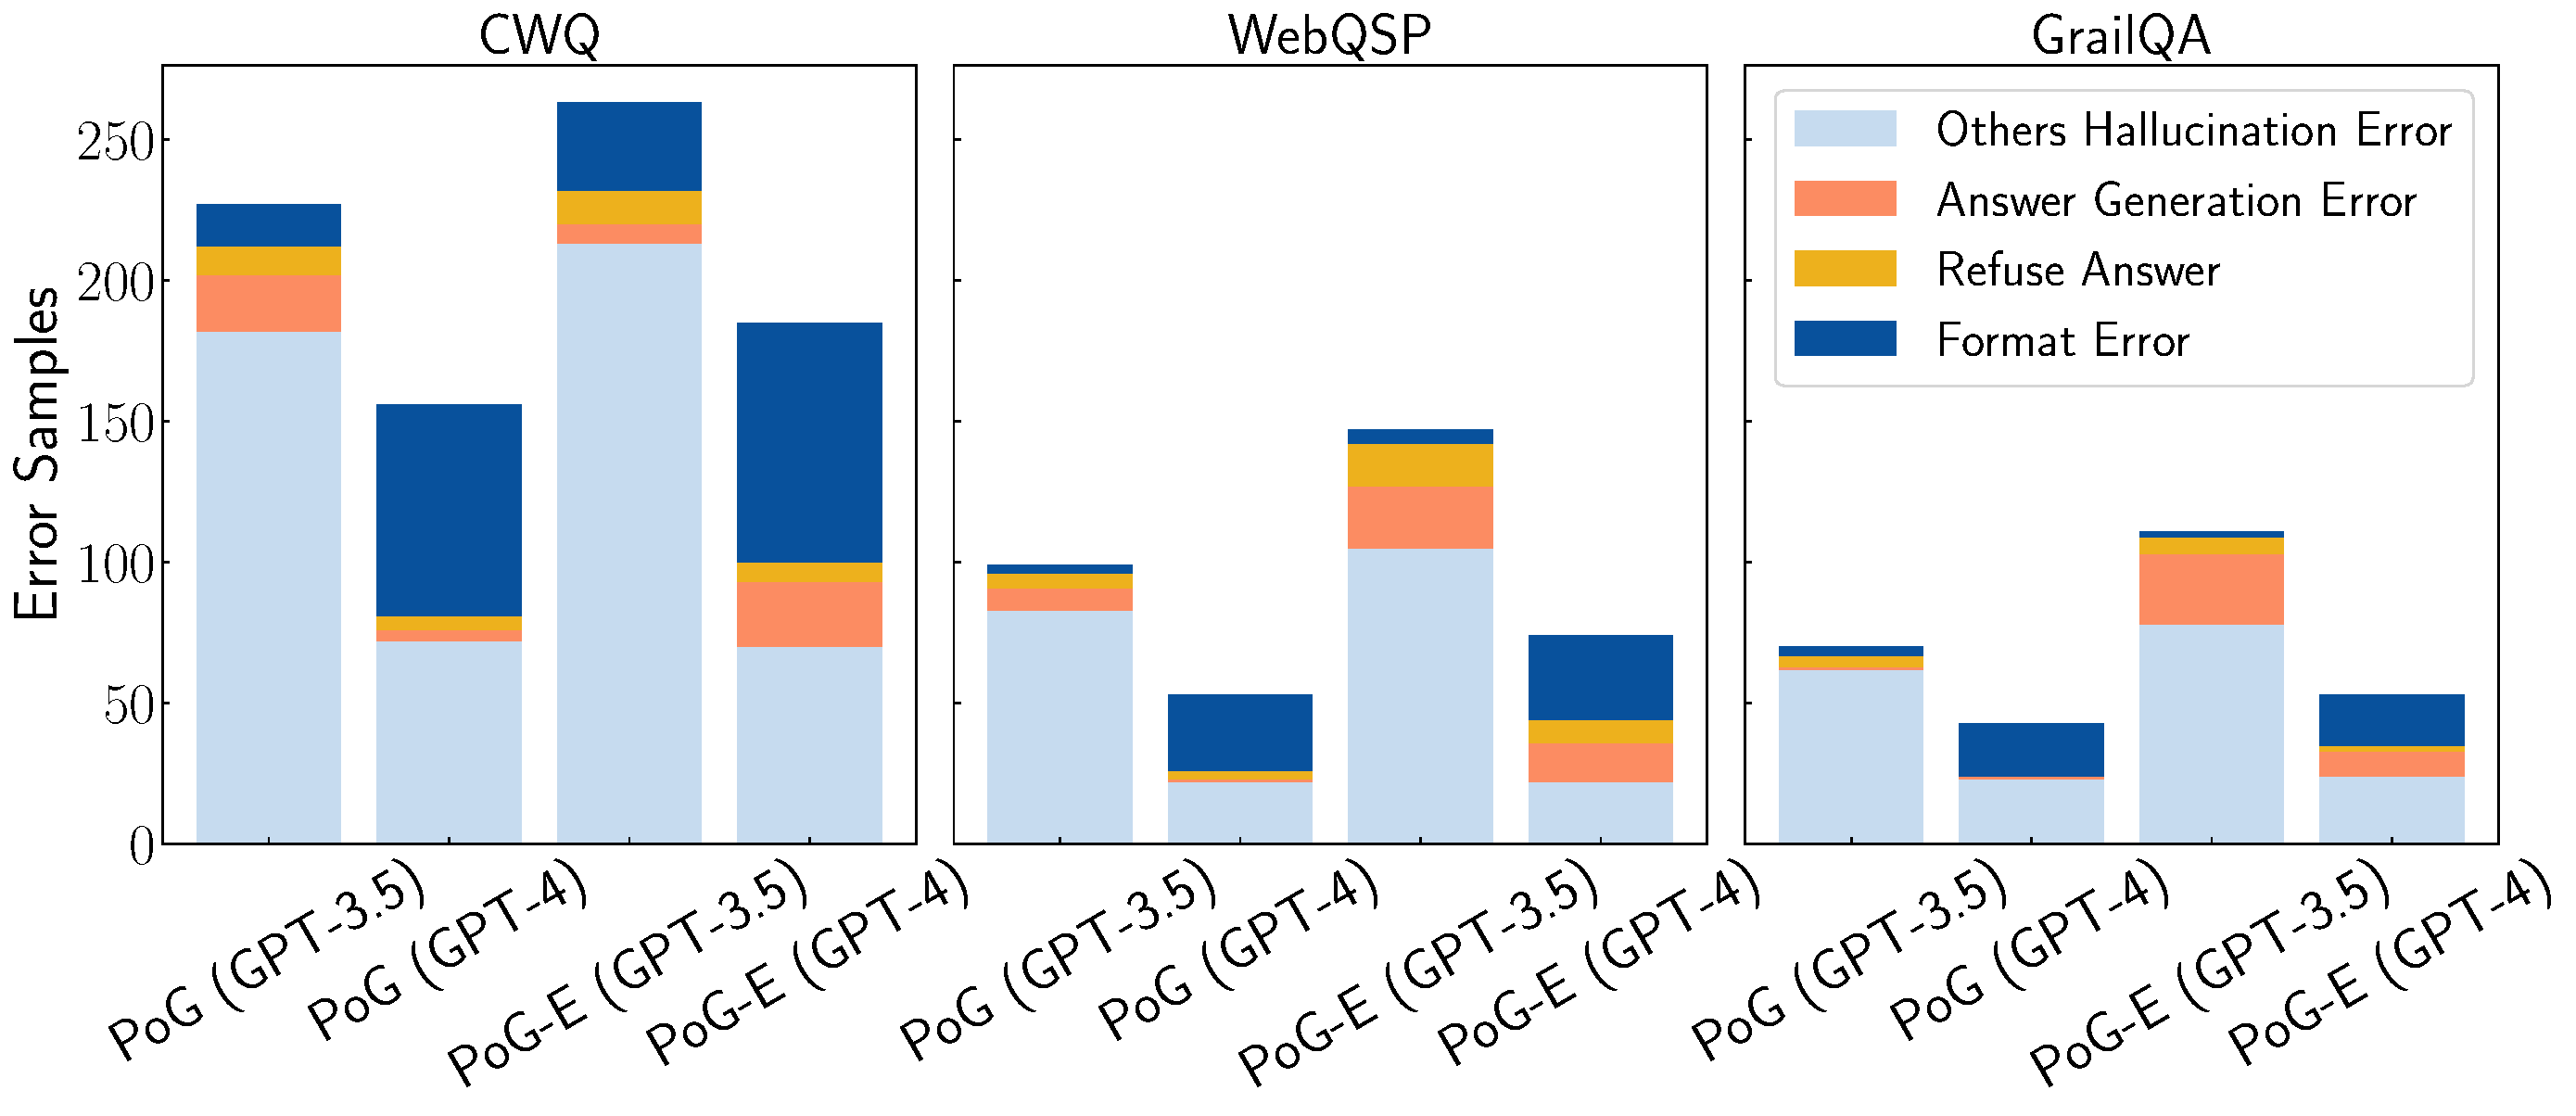
\includegraphics[width=1\linewidth]{graphs/error_analysis_cwq_three_datasets.pdf}
    \caption{The error instances and categories of PoG and PoG-E in the CWQ, WebQSP, and GrailQA datasets.}
    \label{fig:exp:error_analysis}
\end{figure}

% \newpage
\subsection{Efficiency Analysis}\label{appendix:exp:llm_calls}
\myparagraph{LLM calls cost analysis}
To evaluate the cost and efficiency of utilizing LLMs, we conducted an analysis of LLM calls on the CWQ, WebQSP, and GrailQA datasets. Initially, we examined the proportion of questions answered with varying numbers of LLM calls, as depicted in Figure \ref{fig:LLM_call_percentage}. The results indicate that the majority of questions are answered within nine LLM calls across all datasets, with approximately 80\% and 50\% of questions being resolved within six calls on CWQ and WebQSP, respectively. These findings demonstrate PoG's efficiency in minimizing LLM usage costs.
Furthermore, we compared the average number of LLM calls required by PoG with the current SOTA method, ToG \cite{tog1.0sun2023think}, as shown in Table \ref{fig:llmcall_vs_tog}. 
Since we utilized identical datasets for WebQSP, GrailQA, Simple Questions, and WebQuestions, we report the ToG results from their paper. The comparison reveals that PoG achieves comparable or superior accuracy while reducing the number of LLM calls by up to 40\% on the GrailQA dataset compared to ToG. This improvement is attributed to PoG's dynamic exploration strategy, which avoids starting from scratch, and its effective use of graph structures to prune irrelevant information, thereby significantly decreasing computational costs.

\begin{figure}[h]
    \centering
    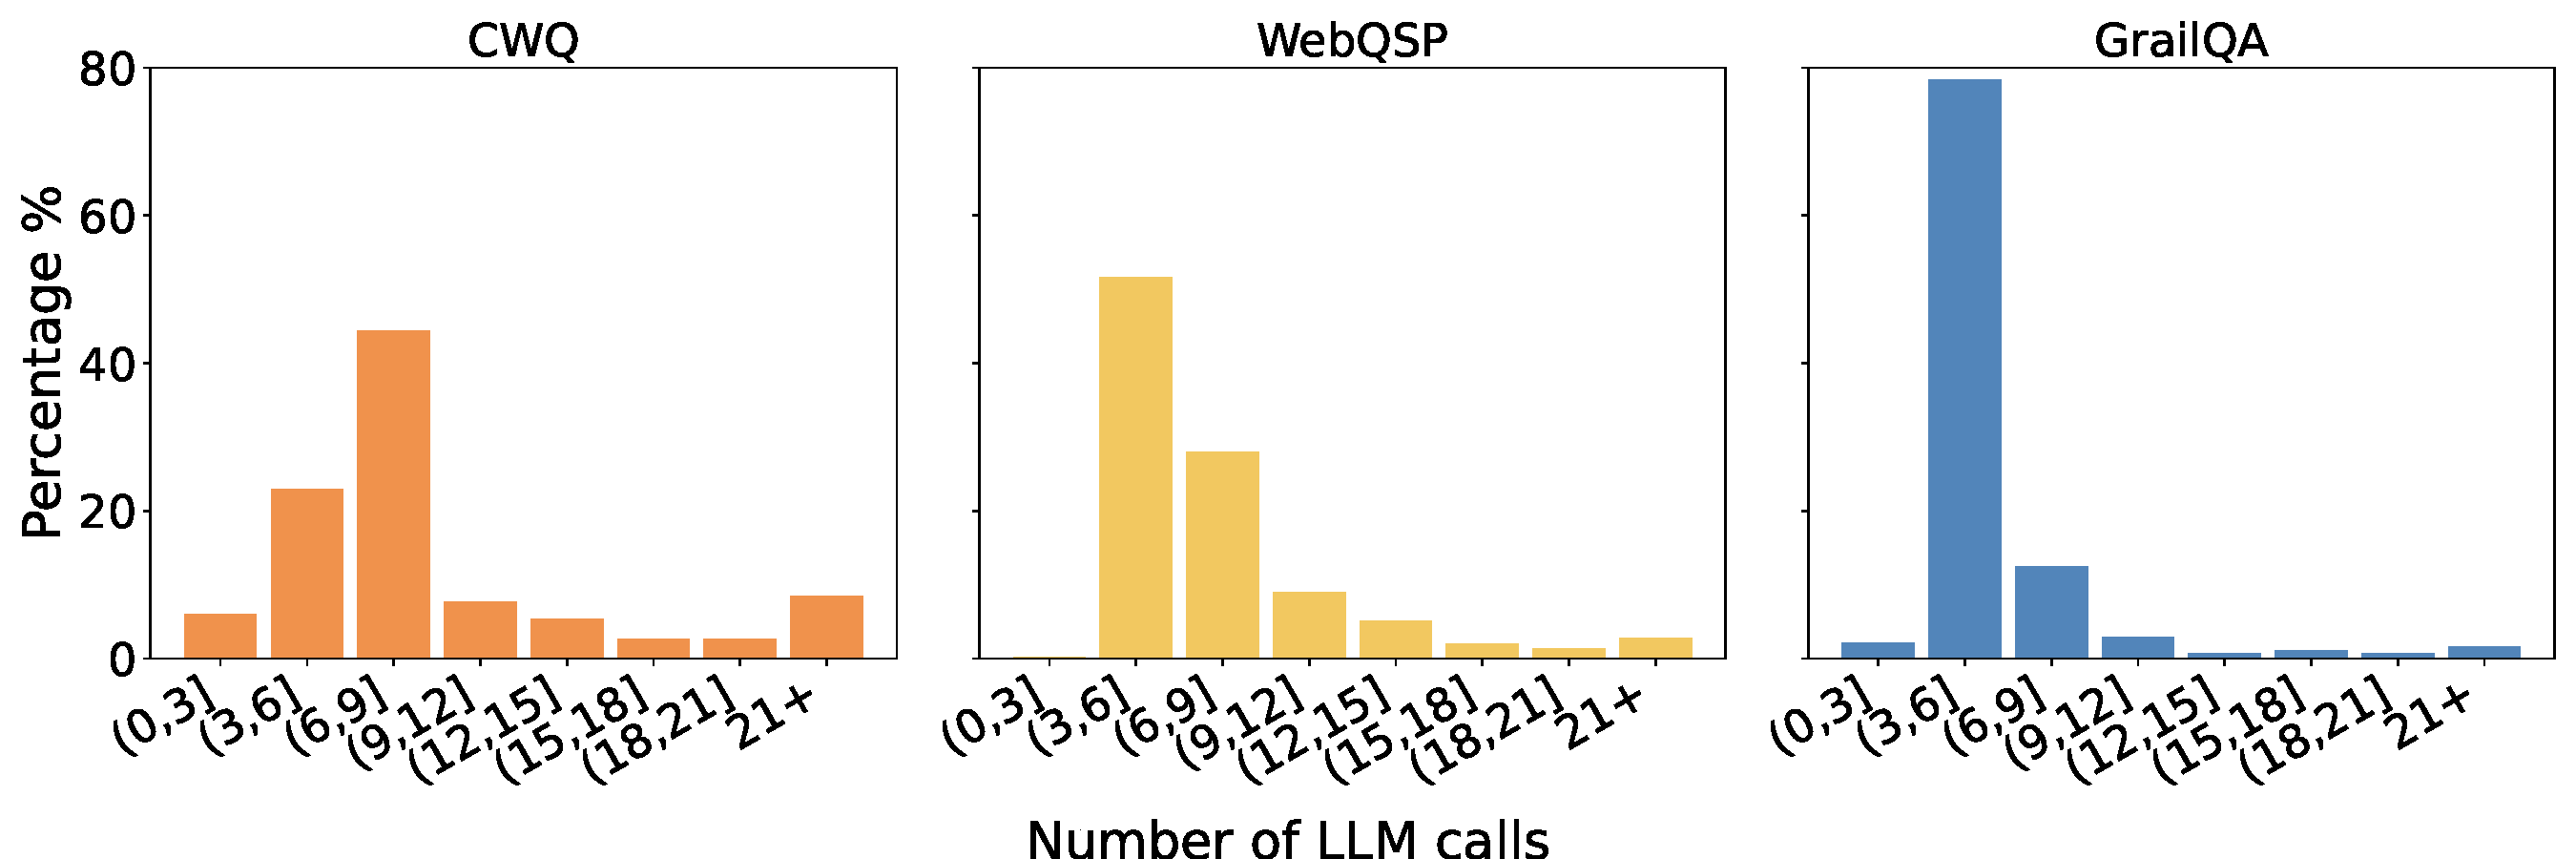
\includegraphics[width=1\linewidth]{graphs/LLM_Calls.pdf}
    
    \caption{The proportion of question of PoG and PoG-E by different LLM Calls among CWQ, WebQSP, and GrailQA datasets}
    \label{fig:LLM_call_percentage}
\end{figure}
% Please add the following required packages to your document preamble:
% \usepackage{booktabs}
% Please add the following required packages to your document preamble:
% \usepackage{booktabs}
\begin{table}[h]

\caption{Average LLM calls per question of PoG and ToG among all datasets.}\label{fig:llmcall_vs_tog}
\setlength\tabcolsep{1 pt}
\resizebox{0.95\columnwidth}{!}{
\begin{tabular}{@{}cccccc@{}}
\toprule
\textbf{Method} & \textbf{CWQ}           & \textbf{WebQSP}       & \textbf{GrailQA}   & \textbf{Simple Questions} & \textbf{WebQuestions}    \\ \midrule
\textbf{PoG}    & \textbf{10.7} & \textbf{8.3} & \textbf{6.5} & \textbf{6.1} & \textbf{9.3}\\
\textbf{ToG}    & -             & 11.2         & 10.6  & 8.7  & 10.5         \\ \bottomrule
\end{tabular}
}
\end{table}

% \myparagraph{Running time analysis}
% To better illustrate the efficiency performance of PoG, we have conducted extensive evaluations focusing on average accuracy, LLM call frequency, and running time on the multi-hop question datasets GrailQA and CWQ. The Table \ref{fig:running_cost_analysis} presents the performance of ToG and PoG with different beam search strategies.
% The result indicates, while improving accuracy may slightly increase runtime, our experiments show that PoG maintains an acceptable balance. PoG can reduce LLM call costs by up to 53.5\% while boosting accuracy by as much as 33.4\%. Within the PoG framework, users can select the most suitable variant based on their requirements for accuracy, cost, and runtime. All PoG setting provide significantly lower costs. For example, on the GrailQA dataset, using PoG-B allows users to achieve a 39.6\% reduction in LLM call costs and a 33.1\% improvement in accuracy with only a 1.14\% increase in runtime. A similar trend is also observed in the CWQ dataset.
\newpage
\myparagraph{Running time analysis}
To further evaluate the processing efficiency of PoG, we conducted extensive evaluations focusing on average accuracy, LLM call frequency, and running time on multi-hop question datasets GrailQA and CWQ. The results, presented in Table \ref{fig:running_cost_analysis}, compare the performance of ToG and PoG across various beam search strategies. The data indicate that while higher accuracy slightly increases runtime, PoG effectively balances accuracy with reduced LLM call costs. Specifically, PoG reduces LLM call costs by up to 53.5\% while increasing accuracy by up to 33.4\%. This allows users to tailor the PoG framework to their specific needs regarding accuracy, cost, and runtime. All PoG setting provide significantly lower costs. For instance, on the GrailQA dataset, PoG with 3-step beam search reduces LLM call costs by 39.6\% and improves accuracy by 33.1\%, with only a 1.14\% increase in runtime. A similar trend is also observed in the CWQ dataset.



\begin{table}[h]
\caption{Running time evaluation of ToG and PoG with different beam search methods on CWQ and GrailQA.}\label{fig:running_cost_analysis}
\begin{tabular}{@{}llcc@{}}
% \small
\toprule
\textbf{Model}              & \textbf{Evaluation} & \textbf{CWQ}  & \textbf{GrailQA} \\ 
\midrule
ToG    & Accuracy           & 53.1    & 59.3            \\
                          & Time (s)         & \textbf{78.7}       & \textbf{14.8}         \\
                          & LLM Calls       & 21.3           & 10.1               \\ 
\midrule
PoG              & Accuracy              & \textbf{81.4} & \textbf{92.7}   \\
 & Time (s)         &118.9           & 21.4         \\
                          & LLM Calls   & 9.1           & 6.5             \\
\midrule
PoG              & Accuracy           & 79.8          & 92.4     \\
w/ 3-Step Beam Search  & Time (s)         & 87.5       & 15.0         \\
                          & LLM Calls       & 8.8         & 6.1       \\ 
\midrule
PoG      & Accuracy           & 57.1          & 83.0           \\
w/ Fuzzy Selection                          & Time (s)         & 109.7             & 15.7         \\
                          & LLM Calls       & \textbf{6.8}           & \textbf{4.7}             \\  \bottomrule
\end{tabular}
\end{table}


% Please add the following required packages to your document preamble:
% \usepackage{booktabs}

\newpage
\subsection{Case Study}\label{appendix:exp_case_study}
\myparagraph{Case study: graph reduction and path pruning}
We conducted a case study using the example question presented in Figure \ref{fig:overall} to illustrate the effects of graph pruning and path pruning on the graph structure. Figure \ref{fig:exp:casestudy1}(a) shows the results of graph pruning, where vertices in blue are selected as part of the question subgraph, and vertices in black are pruned. In this sample, the number of entities is reduced from 16,740 to 1,245, resulting in a 92\% reduction of vertices.
Figures \ref{fig:exp:casestudy1}(b) and \ref{fig:exp:casestudy1}(c) demonstrate the question subgraph induced by the blue vertices in Figure \ref{fig:exp:casestudy1}(a) and the results after applying fuzzy and precise path selection. In these figures, vertices in blue represent the selected entity after each pruning, vertices in yellow represent the topic entities, and the vertex in red denotes the final answer entity.
From these graphs, we observe that utilizing the graph structure allows for the rapid pruning of irrelevant vertices, ensuring that the reasoning paths remain faithful and highly relevant to the question since all vertices within the question subgraph are interconnected with all topic entities, thereby maintaining the integrity and relevance of the reasoning process.
\begin{figure}[h]
    \begin{subfigure}{0.49\linewidth}
           \centering
           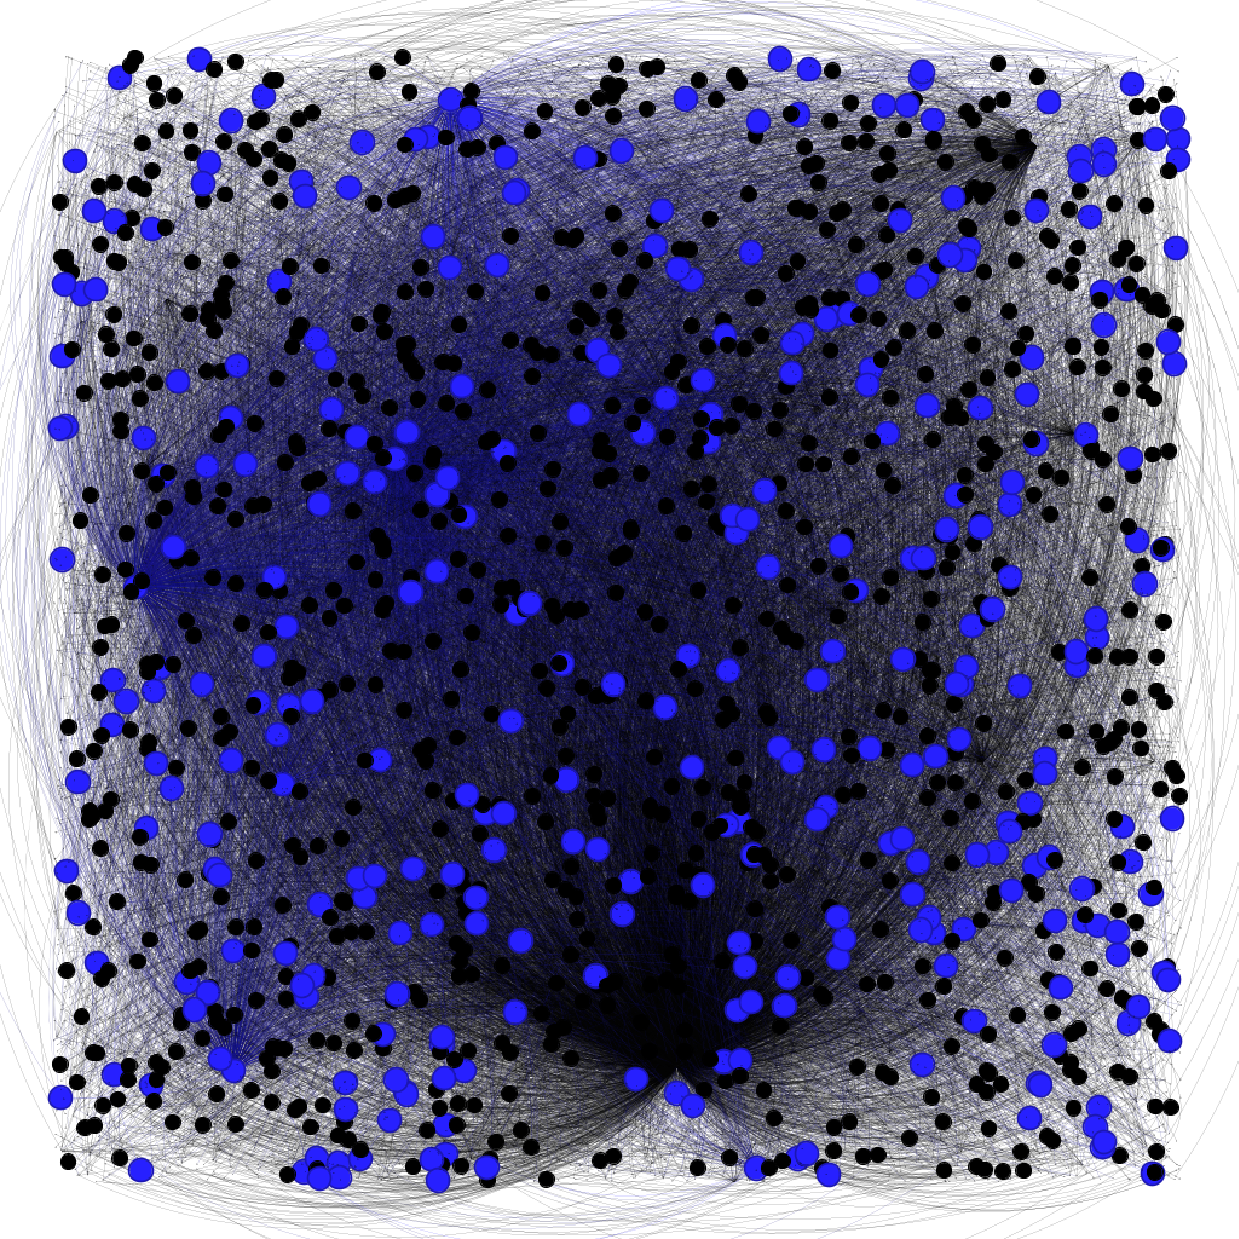
\includegraphics[width=1\linewidth]{graphs/QPathgraph2.pdf}
           
           \caption{Graph pruning}
    \end{subfigure}
    \begin{subfigure}{0.49\linewidth}
           \centering
           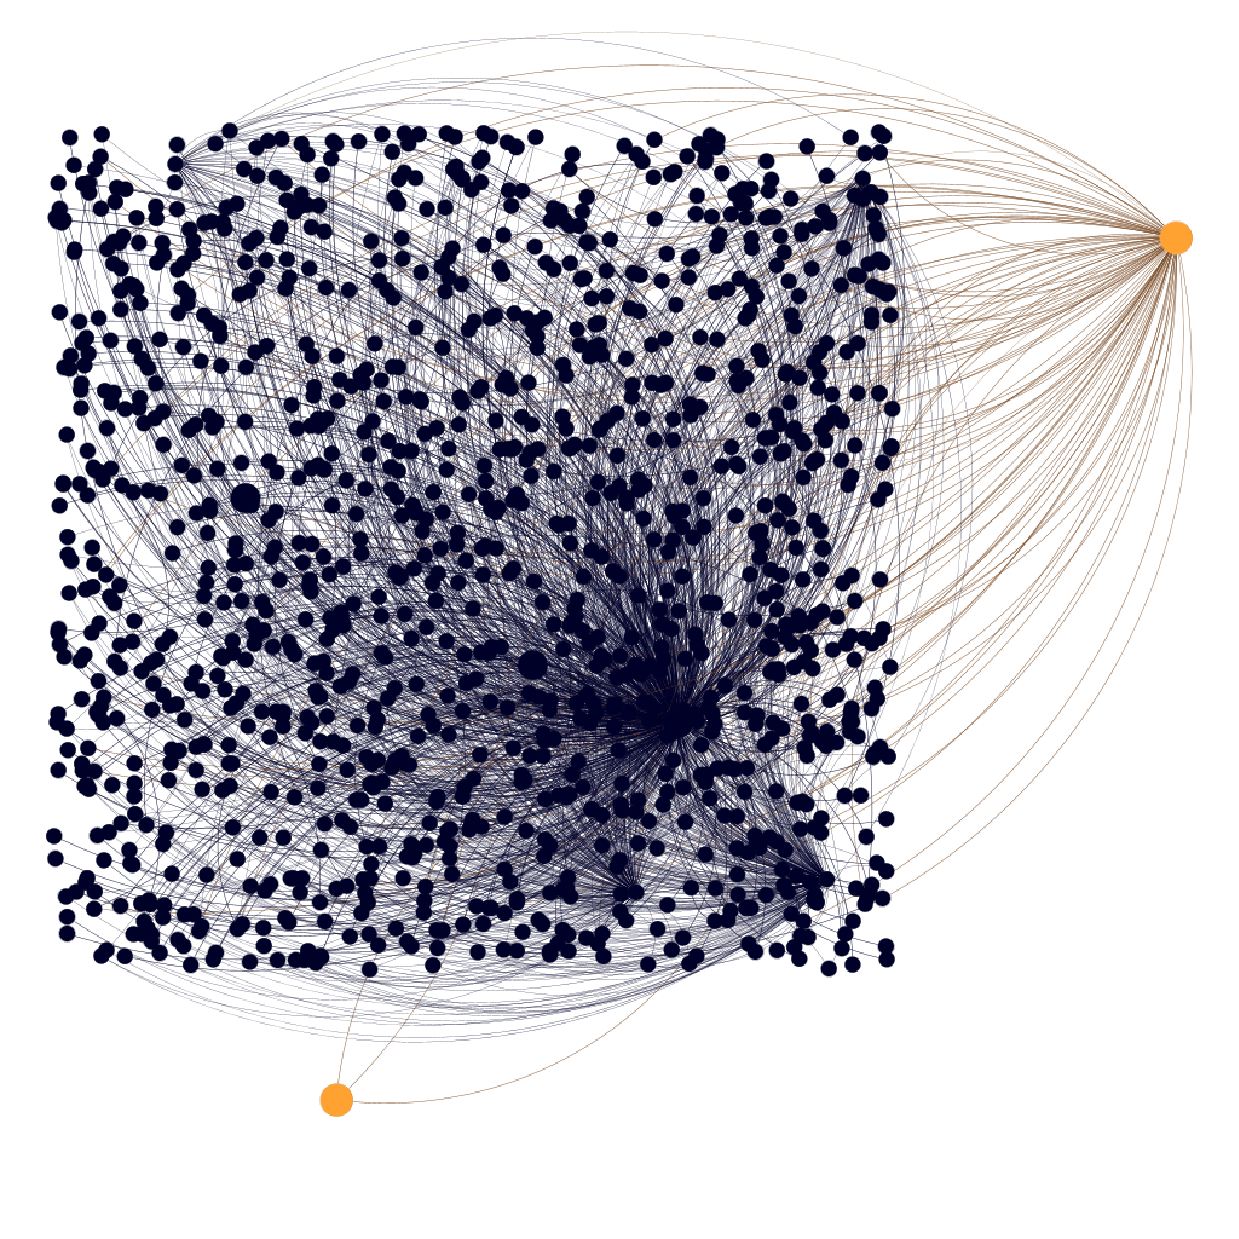
\includegraphics[width=1\linewidth]{graphs/path_graph.pdf}
           
           \caption{Question subgraph}
    \end{subfigure}
    \begin{subfigure}{0.49\linewidth}
           \centering
           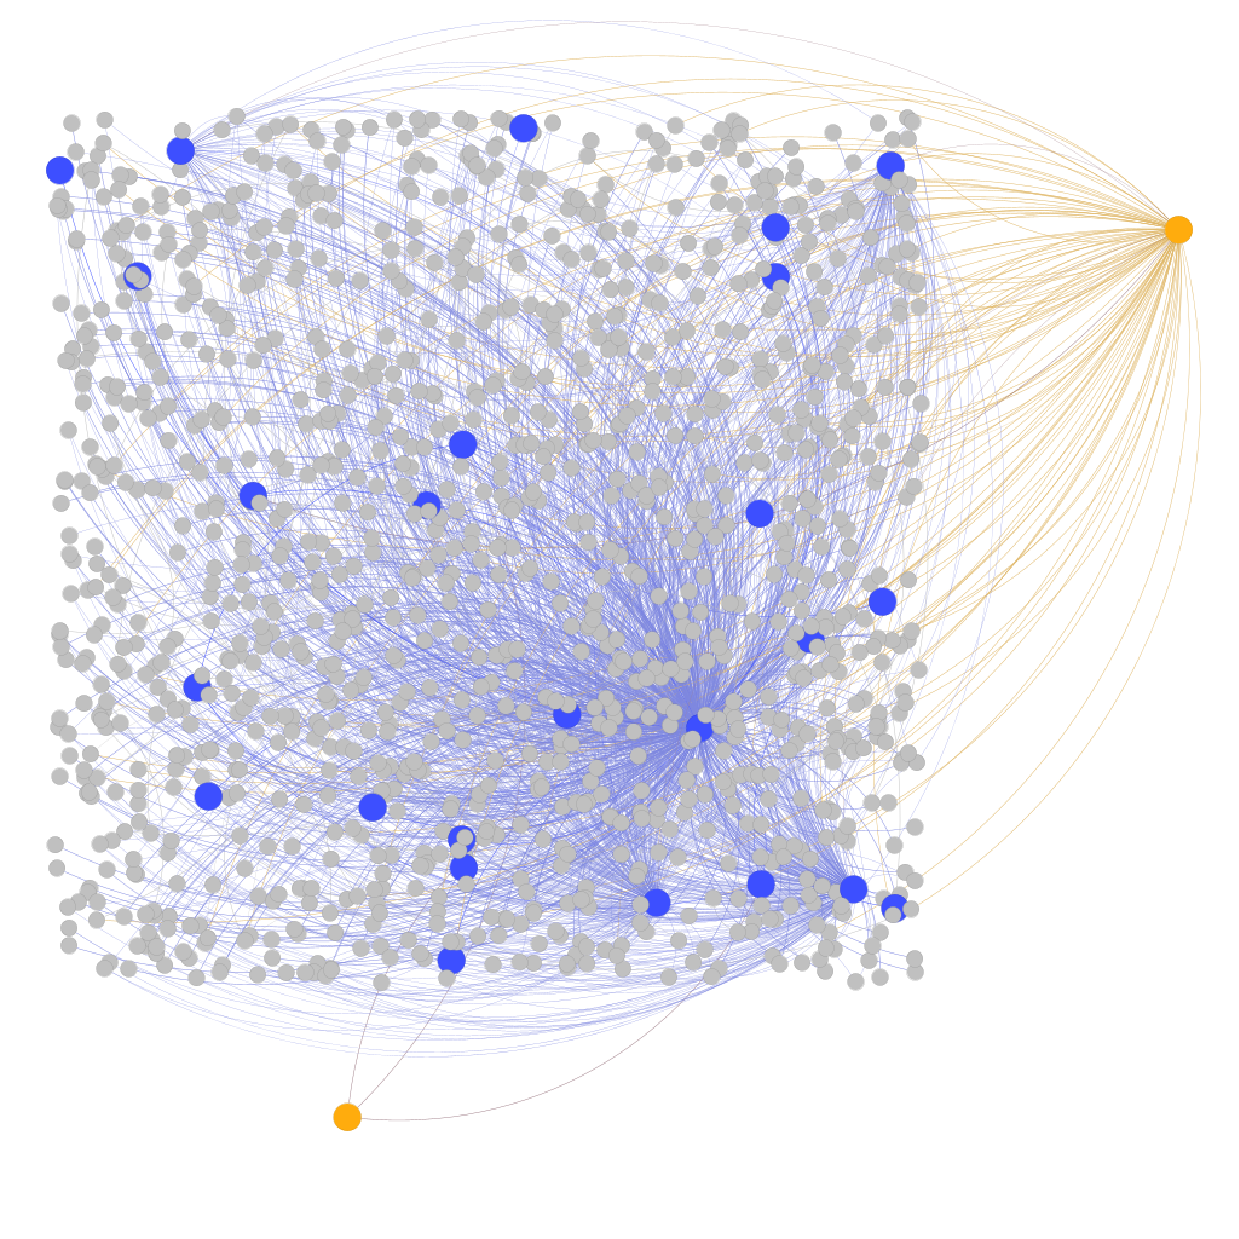
\includegraphics[width=1\linewidth]{graphs/beam_search_1.pdf}
           
           \caption{Fuzzy selection}
    \end{subfigure}
    \begin{subfigure}{0.49\linewidth}
           \centering
           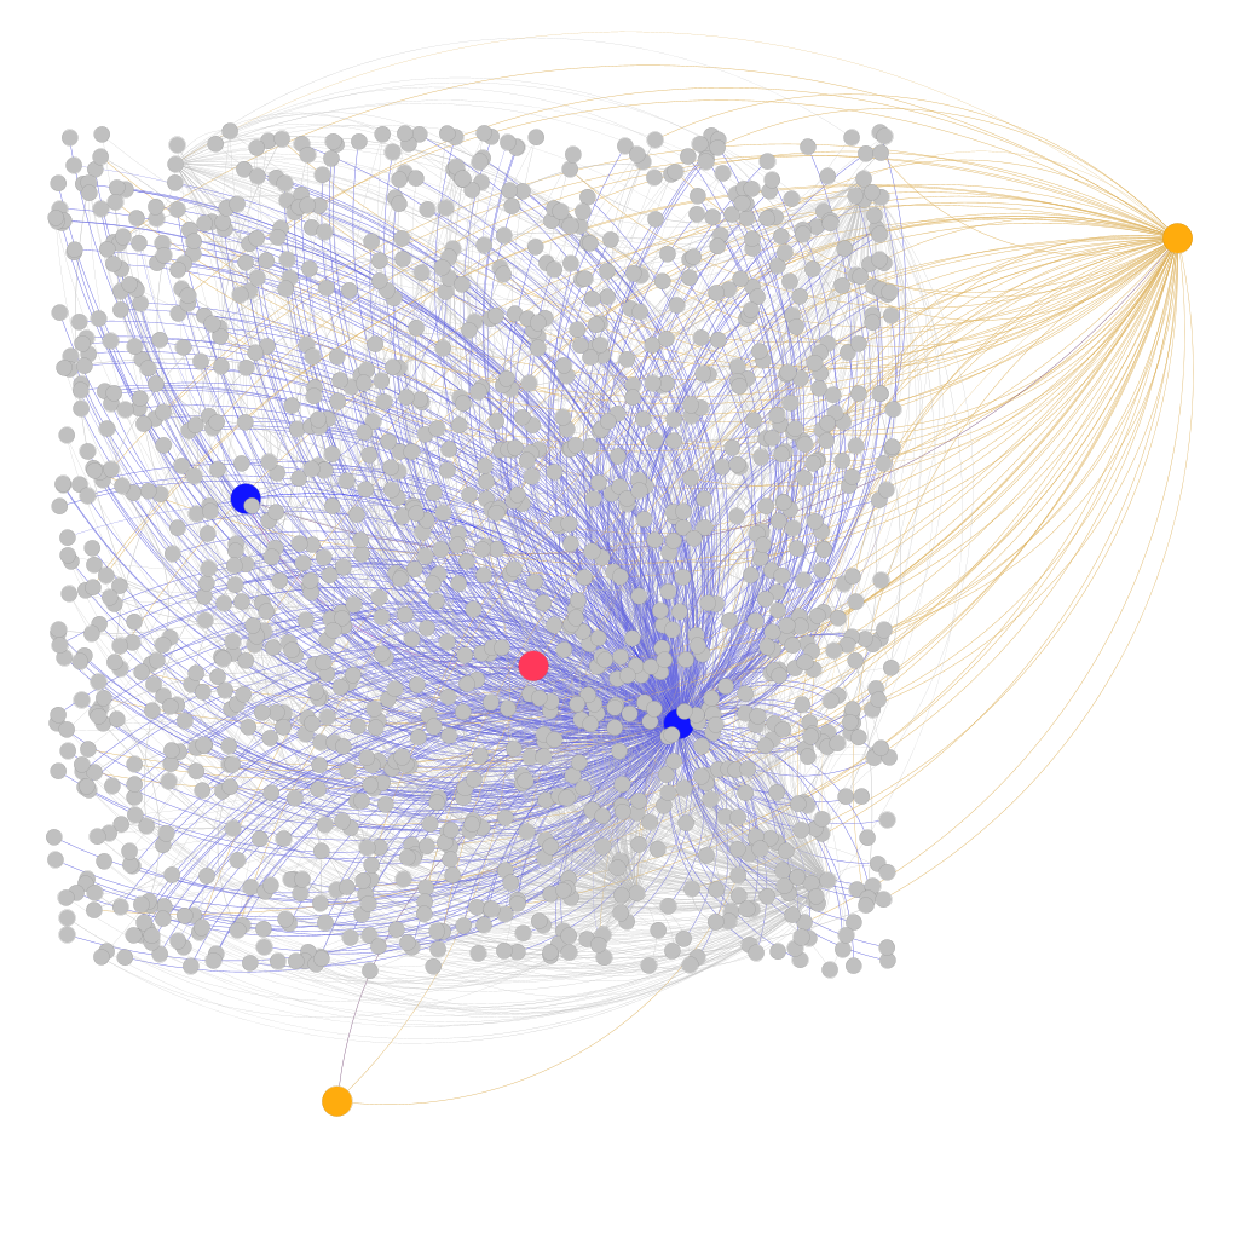
\includegraphics[width=1\linewidth]{graphs/answer.pdf}
           
           \caption{Precise selection}
    \end{subfigure}
    
\caption{Visualization of graph reduction and Path selection.}\label{fig:exp:casestudy1}
\end{figure}




\myparagraph{Case study: interpretable reasoning}
In this section, we present Table \ref{fig:exp:case:interpre}, which illustrates PoG's interpretability through case studies involving questions with one, two, and three entities. These examples demonstrate PoG's effectiveness in handling multi-entity and multi-hop tasks by providing clear and understandable reasoning paths that lead to accurate answers.

\begin{table*}[]
\centering
\vspace{4mm}
\caption{Examples of faithful and interpretable reasoning of PoG.} \label{fig:exp:case:interpre}
% 
\label{tab:case_int}
\begin{tabularx}{0.9\textwidth}{@{}p{3cm}X@{}} 
\toprule
\textbf{Field} & \textbf{Content} \\ 
\midrule
\textbf{Question} & Lou Seal is the mascot for the team that last won the World Series when? \\ 
\textbf{Answer} & 2014 World Series \\
\textbf{Topic Entity} & \textbf{Lou Seal} \\
\toprule
\textbf{LLM indicator} & "\textbf{Lou Seal}" - mascot for - team - last won - World Series - when \\
\textbf{Split Question} & split\_question 1: What team is "Lou Seal" the mascot for? \\

& split\_question 2: When did the last World Series win occur for the team with Lou Seal as the mascot?\\
\toprule
\textbf{Reasoning Path} & \{\textbf{Lou Seal}\} $\rightarrow$ sports.mascot.team $\rightarrow$ \{San Francisco Giants\} $\rightarrow$ sports.sports\_team.championships $\rightarrow$ \{\textcolor{red}{\textbf{2014 World Series}}, 2012 World Series, 2010 World Series\} \\
\toprule
\textbf{PoG answer} & 
\textbf{answer}: \{\textcolor{red}{\textbf{2014 World Series}}\} \\

 & \textbf{reason}: From the given path \{Lou Seal\} $\rightarrow$ sports.mascot.team $\rightarrow$ \{San Francisco Giants\}, \{San Francisco Giants\} is the team that "Lou Seal" serves as the mascot for. From \{San Francisco Giants\} $\rightarrow$ sports.sports\_team.championships $\rightarrow$ \{2014 World Series, 2012 World Series, 2010 World Series\}, the last World Series won by the \{San Francisco Giants\} is in \{2014\}. Therefore, the provided knowledge graph path is sufficient to answer the overall question, and the answer is \{2014 World Series\}.\\
\bottomrule


\midrule
\textbf{Question} & What European Union country sharing borders with Germany contains the Lejre Municipality? \\ 
\textbf{Answer} & Denmark \\
\textbf{Topic Entity} & \textbf{\{Germany, Lejre Municipality\}} \\
\toprule
\textbf{LLM indicator} & "\textbf{Lejre Municipality}" – contained by - European Union country (answer)- shares borders with-"\textbf{Germany}" \\
\textbf{Split Question} & split\_question 1: What European Union country shares borders with "Germany"? \\
& split\_question 2: What country contains the Lejre Municipality?\\
\toprule
\textbf{Reasoning Path} &\{\textbf{Lejre Municipality}\} $\rightarrow$ location.administrative\_division.country $\rightarrow$ \{\textcolor{red}{\textbf{Denmark}}\} $\rightarrow$ location.location.containedby $\rightarrow$ \{Eurasia\} $\rightarrow$ location.location.contains $\rightarrow$ \{\textbf{Germany}\}, \\
&\{\textbf{Lejre Municipality}\} $\rightarrow$ location.administrative\_division.country $\rightarrow$ \{\textcolor{red}{\textbf{Denmark}}\} $\rightarrow$ base.locations.countries. continent $\rightarrow$ \{Europe\} $\rightarrow$ location.location.contains $\rightarrow$ \{Western Europe\} $\rightarrow$ location.location.contains $\rightarrow$ \{\textbf{Germany}\}\\
\toprule
\textbf{PoG answer} & 
\textbf{answer}: \{\textcolor{red}{\textbf{Denmark}}\} \\

 & \textbf{reason}: From \{Denmark\} $\rightarrow $ location.location.containedby $\rightarrow$ \{Eurasia\} $\rightarrow$location.location.contains $\rightarrow$ \{Germany\}, Denmark is European Union country shares borders with "Germany". From \{Lejre Municipality\} $\rightarrow$ location.administrative\_division.country $\rightarrow$ \{Denmark\}, Denmark is a country contains the Lejre Municipality Both paths lead to Denmark, which is the European Union country sharing borders with Germany and containing the Lejre Municipality. Therefore, the provided knowledge graph path is sufficient to answer the main question, and the answer is \{Denmark\}.\\

\bottomrule


\midrule
\textbf{Question} & What Central Tiem Zone continent do the Falkland Islands belong to? \\ 
\textbf{Answer} & Americas \\
\textbf{Topic Entity} & \textbf{\{Falkland Islands, Continent, Central Time Zone\}} \\
\toprule
\textbf{LLM indicator} & answer("\textbf{Central Time Zone}") – owns - answer("\textbf{Continent}")- located contain -"\textbf{Falkland Islands}" \\
\textbf{Split Question} & split\_question 1:What continent do the Falkland Islands belong to? \\

& split\_question 2: What Central Time Zone does the continent belong to?\\
\toprule
\textbf{Reasoning Path} &\{\textbf{Central Time Zone}\} $\rightarrow$ time.time\_zone.locations\_in\_this\_time\_zone $\rightarrow$ \{\textcolor{red}{\textbf{Americas}}\} $\rightarrow$ common.topic.not able\_types  $\rightarrow$ \{\textbf{Continent}\} $\rightarrow$ common.topic. notable\_types  $\rightarrow$ \{Americas\} $\rightarrow$ location.location.con tains  $\rightarrow$\{ \textbf{Falkland Islands}\}\\
\toprule
\textbf{PoG answer} & 
\textbf{answer}: \{\textcolor{red}{\textbf{Americas}}\} \\

 & \textbf{reason}: From \{Continent\} $\rightarrow$ common.topic.notable\_types  $\rightarrow$ \{Americas\} $\rightarrow$ location.location. contains  $\rightarrow$\{ Falkland Islands\}, Americas  is the continent Falkland Islands belong to.
From \{Central Time Zone\} $\rightarrow$ time.time\_zone.locations\_in\_this\_time\_zone $\rightarrow$ \{Americas\} $\rightarrow$ common.topic. notable\_types  $\rightarrow$ \{Continent\}. Americas is the Central Time Zone.
Therefore, the provided knowledge graph path is sufficient to answer the overall question, and the answer is \{Americas\}.
\\

\bottomrule
\end{tabularx}
\end{table*}


\newpage
\section{Experiment Details}
\label{appen:dataset_details}
% Please add the following required packages to your document preamble:
% \usepackage{booktabs}
% The statistics of the datasets used in this paper are shown in Table \ref{table:datatsets}.
% We also provide a detailed result table for each dataset, shown in Table 10 to Table 18, illustrating the enhancements of ToG compared to the previous fine-tuning-based and prompting-based relevant works. For WebQSP, GrailQA, WebQuestion, ChatGPT-based PoG leads a new state-of-the-art.
% For CWQ, GPT4-based PoG leads a new state-of-the-art.
% Furthermore, GPT-4-based PoG exceeded the fine-tuning-based approaches on all Multi-Hop
% KBQA datasets, where on datasets CWQ, Simple Questions, PoG close to the state-of-the-art (83.9\%).


\myparagraph{Experiment datasets} To evaluate PoG's capability in multi-hop knowledge-intensive reasoning tasks, we assess it on four KBQA datasets: three multi-hop datasets (CWQ \cite{talmor-berant-2018-web}, WebQSP \cite{yih-etal-2016-value}, GrailQA \cite{grailqa}) and one single-hop dataset (SimpleQuestions \cite{simplequestions}). Additionally, to examine PoG on more general tasks, we include an open-domain QA dataset, WebQuestions.
For the evaluation of large datasets such as CWQ, GrailQA, and SimpleQuestions, we utilize a random sample of 1,000 test cases from CWQ and employ the 1,000 samples previously reported by ToG \cite{tog1.0sun2023think} to facilitate a comparison with the SOTA while also minimizing computational costs. Freebase serves as the background knowledge graph for all datasets, which encompasses approximately 88 million entities, 20,000 relations, and 126 million triples \cite{rogluo2023reasoning, freebase}. The statistics of the datasets utilized in this study are detailed in Table \ref{fig:appendix:dataset}. The source code has been publicly available\footnote{https://github.com/SteveTANTAN/PoG}.


\myparagraph{Baselines} 
Inspired by ToG \cite{tog1.0sun2023think}, we compare our method with standard prompting (IO), Chain-of-Thought (CoT), and Self-Consistency (SC) promptings with six in-context exemplars and "step-by-step" reasoning chains. For each dataset, we also include previous SOTA works for comparison. 
For a fair play, we compare with previous SOTA among all prompting-based methods and previous SOTA among all methods respectively.
Since ToG is the current SOTA prompting-based method, we directly refer to their results and those of other baselines reported in their paper for comparisons.


\myparagraph{Experimental implementation}
Leveraging the plug-and-play convenience of our framework, we experiment with two LLMs: GPT-3.5 and GPT-4. We use the OpenAI API to access GPT-3.5 (GPT-3.5-turbo) and GPT-4. Aligning with ToG, we set the temperature parameter to 0.4 during the exploration process (to increase diversity) and to 0 during the reasoning process (to ensure reproducibility). The maximum token length for generation is set to 256.
In all experiments, we set both $W_{\max}$ and $D_{\max}$ to 3 for beam search. All the experiments are conducted on a machine with Intel Xeon
Gold 6248R CPU, Nvidia A5000 GPU and 512GB memory.


% In addition, comprehensive results are presented for each data set,
% highlighting the advancements achieved by ToG over prior fine-tuning-based and prompting-based methods. Notably, for the datasets WebQSP, GrailQA, and WebQuestions, PoG based on ChatGPT establishes a new state-of-the-art. Similarly, for CWQ, PoG powered by GPT-4 sets a new benchmark.
% Moreover, GPT-4-based PoG surpasses fine-tuning-based methods across all Multi-Hop KBQA datasets. Specifically, in datasets such as CWQ and Simple Questions, PoG's performance approaches the state-of-the-art, achieving an accuracy of 83.9\%.



\begin{table}[H]
% \caption{The statistics of the datasets used in this paper. $^\dagger$ denotes we randomly selected 1,000 samples from the CWQ test set to constitute the testing set owing to the abundance of test samples.
% $^\ast$ denotes wee utilize the 1,000 samples reported by ToG\cite{tog1.0sun2023think} to compare with the state-of-the-art.}\label{fig:appendix:dataset}
% \vspace{mm}
\caption{
Statistics of the datasets used in this paper. 
$^\dagger$ denotes we randomly select 1,000 samples from the CWQ test set to create the experiment testing set due to the abundance of test samples.
$^\ast$ denotes that we utilize the 1,000 samples reported by ToG \cite{tog1.0sun2023think} to compare with the state-of-the-art.
}\label{fig:appendix:dataset}

\setlength\tabcolsep{1 pt}
\resizebox{0.95\columnwidth}{!}{
% Please add the following required packages to your document preamble:
% \usepackage{booktabs}
\begin{tabular}{@{}cccc@{}}
\toprule
Dataset             & Answer Format & Test  & Train \\ \midrule
ComplexWebQuestions (CWQ) $^\dagger$ & Entity        & 1,000 & 27,734                    \\
WebQSP              & Entity/Number & 1,639 &  3,098                      \\
GrailQA$^\ast $           & Entity/Number & 1,000 & 44,337                      \\
Simple Question$^\ast$    & Entity/Number & 1,000 &  14,894                       \\
WebQuestions        & Entity/Number & 2,032 & 3,778                      \\ \bottomrule
\end{tabular}
}
\end{table}

\newpage
\section{SPARQL}\label{appendix:aparql}
This section outlines the pre-defined SPARQL queries used for interacting with the knowledge graph and constructing graphs for our experiments. 

% \subsubsection{Pre-defined Sparql}
\subsection{1-hop Entity and Relation Search}\label{appendix:1_hop_e_r_search}
To facilitate the retrieval of 1-hop neighbors of entities within the Freebase Knowledge Graph, we have predefined a SPARQL query. This query is designed to be executed by simply substituting the appropriate ID for the query entity ID. It returns the connected entities' IDs and their associated relations' IDs, indicating whether the connected entity is at the tail or the head of the relation.

\lstset{language=SPARQL}
\begin{lstlisting}
PREFIX ns: <http://rdf.freebase.com/ns/>
SELECT ?|\textcolor{cyan}{relation}| ?|\textcolor{red}{connectedEntity}| ?direction
WHERE {
    {
        ns:|\textcolor{purple}{ID}| ?|\textcolor{cyan}{relation}| ?|\textcolor{red}{connectedEntity}| .
        BIND(|\textcolor{olive}{"tail"}| AS ?direction)
    }
    UNION
    {
        ?|\textcolor{red}{connectedEntity}| ?|\textcolor{cyan}{relation}| ns:|\textcolor{purple}{ID}| .
        BIND(|\textcolor{orange}{"head"}| AS ?direction)
    }
}
\end{lstlisting}

% \newpage
\subsection{Short Textual Description}\label{appendix:short_D}
The following predefined function implements the retrieval of short textual descriptions, $\mathcal{D}(.)$, for converting the identifiers (IDs) of entities or relations into natural language descriptions.



\lstset{language=SPARQL}
\begin{lstlisting}
PREFIX ns: <http://rdf.freebase.com/ns/>
SELECT DISTINCT ?|\textcolor{cyan}{tailEntity}|
WHERE {
    {    
        ?|\textcolor{brown}{entity}| ns:type.object.name ?|\textcolor{cyan}{tailEntity}| .
        FILTER(?|\textcolor{brown}{entity}| = ns:|\textcolor{purple}{ID}|)  
    }  
    UNION
    {    
        ?|\textcolor{brown}{entity}| <http://www.w3.org/2002/07/owlsameAs> ?|\textcolor{cyan}{tailEntity}| .    
        FILTER(?|\textcolor{brown}{entity}| = ns:|\textcolor{purple}{ID}|)  
    }
}

\end{lstlisting}

% \subsubsection{1-hop Subgraph Search}
% To realize the subgraph detection in section \ref{method:1.1subgraphD}, we implement the 1-hop subgraph detection, which is the combination of previous Sparql function in appendix \ref{appendix:1_hop_e_r_search} \& \ref{appendix:short_D}
% In this function, by given the query entity ID, we can obtain its 1-hop neighbors' ID, natural language name, and their associated relations, indicating whether the connected entity is at the tail or the head of the relation, in one Sparql query. 

\newpage
\subsection{1-hop Subgraph Search}
To facilitate subgraph detection in Section \ref{method:initialization}, we implement the 1-hop subgraph detection feature by integrating SPARQL functions described in Appendix \ref{appendix:1_hop_e_r_search} and \ref{appendix:short_D}. The purpose of this function is to retrieve, in a single SPARQL query, the 1-hop neighbors of a given query with their IDs, natural language names, and connected relationships, specifying whether the connected entity is at the tail or the head of the relationship.
\lstset{language=SPARQL}
\begin{lstlisting}
PREFIX ns: <http://rdf.freebase.com/ns/>
SELECT ?|\textcolor{cyan}{relation}| ?|\textcolor{red}{connectedEntity}| ?|\textcolor{teal}{connectedEntityName}| ?direction
WHERE {
    {
        ns:|\textcolor{purple}{ID}| ?|\textcolor{cyan}{relation}| ?|\textcolor{red}{connectedEntity}| .
        OPTIONAL {
            ?|\textcolor{red}{connectedEntity}| ns:type.object.name ?name .
            FILTER(lang(?name) = 'en')
        }
        BIND(COALESCE(?name, |\textcolor{black}{"Unnamed Entity"}|) AS ?|\textcolor{teal}{connectedEntityName}|)
        BIND(|\textcolor{olive}{"tail"}| AS ?direction)
    }
    UNION
    {
        ?|\textcolor{red}{connectedEntity}| ?|\textcolor{cyan}{relation}| ns:|\textcolor{purple}{ID}| .
        OPTIONAL {
            ?|\textcolor{red}{connectedEntity}| ns:type.object.name ?name .
            FILTER(lang(?name) = 'en')
        }
        BIND(COALESCE(?name, |\textcolor{black}{"Unnamed Entity"}|) AS ?|\textcolor{teal}{connectedEntityName}|)
        BIND(|\textcolor{orange}{"head"}| AS ?direction)
    }
}
\end{lstlisting}

\newpage
\onecolumn
\section{Prompts}\label{appendix:prompt}
In this section, we detail the prompts required for our main experimental procedures.

\begin{center}
\begin{minipage}{0.7\columnwidth}
    \vspace{2mm}
        \centering
    \begin{tcolorbox}[title=Question Analysis Prompt Template] 
        \small
            % \centering
    You will receive a multi-hop question, which is composed of several interconnected queries, along with a list of topic entities that serve as the main keywords for the question. Your task is to break the question into simpler parts, using each topic entity once and provide a Chain of Thought (CoT) that shows how the topic entities are related. Note: Each simpler question should explore how one topic entity connects to others or the answer. The goal is to systematically address each entity to derive the final answer.
\vspace{5pt}
    
    \texttt{In-Context Few-shot}
\vspace{5pt}
    
    Q: \{Query\} 
    
    Topic Entity: \{Topic Entity\} 
    
    A: 
    \end{tcolorbox}
    % \vspace{1mm}
    \vspace{2mm}

\end{minipage}
\end{center}

\begin{center}
\begin{minipage}{0.7\columnwidth}
    % \centering
    \vspace{2mm}
    \begin{tcolorbox}[title=LLM Supplement Prompt Template]~\label{prompts_LLM_Supplement}
        \small
Using the main question, a possibly uncertain chain of thought generated by a language model, some related split questions, paths from the "Related\_paths" section, and main topic entities:
please first provide three predicted results,
and second offer three possible chains of thought that could lead to these results, using the provided knowledge paths and your own knowledge.
If any answers are unclear, suggest alternative answers to fill in the gaps in the chains of thought, following the same format as the provided examples.

\vspace{5pt}

\texttt{In-Context Few-shot}
\vspace{5pt}

Q: \{Query\} 

Topic Entity: \{Topic Entity\} 

Think Indicator:\{Think Indicator\}

Split Question:\{Split Question\}

A: 
    \end{tcolorbox}
    \vspace{2mm}
\end{minipage}
\end{center}
where \texttt{\{Think Indicator\}, \text{and} \{Split Question\}} are obtained in section \ref{method:initialization}. An indicator example is shown in Figure \ref{fig:overall}.

\begin{center}
    
\begin{minipage}{0.7\columnwidth}
    \centering
    % \vspace{pt}
    \vspace{2mm}
    
    \begin{tcolorbox}[title=Precise Path Select Prompt Template]
        \small
Given a main question, a LLM-generated thinking Cot that considers all the entities, a few split questions that you can use one by one and finally obtain the final answer, and the associated retrieved knowledge graph path, \{set of entities (with id start with "m.")\} -> \{set of relationships\} -> \{set of entities(with id start with "m.")\}, 
Please score and give me the top three lists from the candidate paths set can be highly to be the answer of the question.

\vspace{5pt}
    
\texttt{In-Context Few-shot}

\vspace{5pt}
Q: \{Query\} 

Think Indicator:\{Think Indicator\}

Split Question:\{Split Question\}

Candidate Paths:\{Candidate Paths\}

A: 
\end{tcolorbox}
\vspace{2mm}
\end{minipage}
\end{center}
\texttt{\{Candidate Paths\}} denotes the retrieved reasoning paths $Final_paths$ to be selected in this request which are formatted as a series of structural sentences:

\begin{minipage}{0.99\columnwidth}
    \centering
    $\{e_{0x},...,e_{0z}\}\to r_{1_i} \to \{e_{1x},...,e_{1z}\}\to \dots$ $\to r_{l_j} \to \{e_{lx},...,e_{lz}\}$ 
    \\ $\dots$\\
    $\{e_{0x},...,e_{0z}\}\to r_{1_i} \to \{e_{1x},...,e_{1z}\}\to \dots$ $\to r_{l_j} \to \{e_{lx},...,e_{lz}\}$,
    % \vspace{5pt}
    
\end{minipage}

\noindent where, $i$ and $j$ in $r_{1_i}, r_{1_i}$ represent the $i$-th, $j$-th relation from each relation edge in the clustered question subgraph.
And $e$ is constructed by its ID and natural language name $\mathcal{D}(ID)$.
\vspace{5pt}

\begin{center}
    
\begin{minipage}{0.7\columnwidth}
    % \centering
    \vspace{2mm}
    \begin{tcolorbox}[title=Path Summarizing Prompt Template]
        \small
Given a main question, an uncertain LLM-generated thinking Cot that considers all the entities, a few split questions that you can use one by one and finally obtain the final answer, the associated accuracy retrieved knowledge paths from the Related paths section, and main topic entities.
Your task is to summarize the provided knowledge triple in the Related paths section and generate a chain of thoughts by the knowledge triple related to the main topic entities of the question, which will used for generating the answer for the main question and split question further.
You have to make sure you summarize correctly by using the provided knowledge triple, you can only use the entity with id from the given path and you can not skip in steps.


\vspace{5pt}
    
\texttt{In-Context Few-shot}

\vspace{5pt}
Q: \{Query\} 

Think Indicator:\{Think Indicator\}

Split Question:\{Split Question\}

Related Paths:\{Related Paths\}

A: 
    \end{tcolorbox}
    \vspace{2mm}
\end{minipage}
\end{center}

    % \vspace{5pt}

\noindent\texttt{\{Related\_Paths\}} has the same format with the \texttt{\{Candidate\_Paths\}} before.
    % \vspace{5pt}

\begin{center}
    
\begin{minipage}{0.7\columnwidth}
    % \centering
    \vspace{2mm}
    
    \begin{tcolorbox}[title= Question Answering Evaluation Prompt Template]
        \small
Given a main question, an uncertain LLM-generated thinking Cot that considers all the entities, a few split questions that you can use and finally obtain the final answer, and the associated retrieved knowledge graph path, \{set of entities (with id start with "m.")\} -> \{set of relationships\} -> \{set of entities(with id start with "m.")\}.
Your task is to determine if this knowledge graph path is sufficient to answer the given split question first then the main question. 
If it's sufficient, you need to respond \{Yes\} and provide the answer to the main question. If the answer is obtained from the given knowledge path, it should be the entity name from the path. Otherwise, you need to response \{No\}, then explain the reason. 


\vspace{5pt}
    
\texttt{In-Context Few-shot}

\vspace{5pt}
Q: \{Query\} 

Think Indicator:\{Think Indicator\}

Split Question:\{Split Question\}

Related Paths:\{Related Paths\}

A: 
    \end{tcolorbox}
    \vspace{2mm}
\end{minipage}
\end{center}

\begin{center}

\begin{minipage}{0.7\columnwidth}
    % \centering
    \vspace{2mm}
    \begin{tcolorbox}[title= Question Answering Generation Prompt Template]
        \small
Given a main question, an uncertain LLM-generated thinking Cot that considers all the entities, a few split questions that you can use one by one and finally obtain the final answer, and the associated retrieved knowledge graph path, \{set of entities (with id start with "m.")\} -> \{set of relationships\} -> \{set of entities(with id start with "m.")\}, 
Your task is to generate the answer based on the given knowledge graph path and your own knowledge.

\vspace{5pt}
    
\texttt{In-Context Few-shot}

\vspace{5pt}
Q: \{Query\} 

Think Indicator:\{Think Indicator\}

Split Question:\{Split Question\}

Related Paths:\{Related Paths\}

A: 
    \end{tcolorbox}
    \vspace{2mm}
\end{minipage}
\end{center}


